

\documentclass[11pt,compress,t,notes=noshow]{beamer}\usepackage[]{graphicx}\usepackage[]{color}

\makeatletter
\def\maxwidth{ %
  \ifdim\Gin@nat@width>\linewidth
    \linewidth
  \else
    \Gin@nat@width
  \fi
}
\makeatother

\definecolor{fgcolor}{rgb}{0.345, 0.345, 0.345}
\newcommand{\hlnum}[1]{\textcolor[rgb]{0.686,0.059,0.569}{#1}}%
\newcommand{\hlstr}[1]{\textcolor[rgb]{0.192,0.494,0.8}{#1}}%
\newcommand{\hlcom}[1]{\textcolor[rgb]{0.678,0.584,0.686}{\textit{#1}}}%
\newcommand{\hlopt}[1]{\textcolor[rgb]{0,0,0}{#1}}%
\newcommand{\hlstd}[1]{\textcolor[rgb]{0.345,0.345,0.345}{#1}}%
\newcommand{\hlkwa}[1]{\textcolor[rgb]{0.161,0.373,0.58}{\textbf{#1}}}%
\newcommand{\hlkwb}[1]{\textcolor[rgb]{0.69,0.353,0.396}{#1}}%
\newcommand{\hlkwc}[1]{\textcolor[rgb]{0.333,0.667,0.333}{#1}}%
\newcommand{\hlkwd}[1]{\textcolor[rgb]{0.737,0.353,0.396}{\textbf{#1}}}%
\let\hlipl\hlkwb

\usepackage{framed}
\makeatletter
\newenvironment{kframe}{%
 \def\at@end@of@kframe{}%
 \ifinner\ifhmode%
  \def\at@end@of@kframe{\end{minipage}}%
  \begin{minipage}{\columnwidth}%
 \fi\fi%
 \def\FrameCommand##1{\hskip\@totalleftmargin \hskip-\fboxsep
 \colorbox{shadecolor}{##1}\hskip-\fboxsep
     \hskip-\linewidth \hskip-\@totalleftmargin \hskip\columnwidth}%
 \MakeFramed {\advance\hsize-\width
   \@totalleftmargin\z@ \linewidth\hsize
   \@setminipage}}%
 {\par\unskip\endMakeFramed%
 \at@end@of@kframe}
\makeatother

\definecolor{shadecolor}{rgb}{.97, .97, .97}
\definecolor{messagecolor}{rgb}{0, 0, 0}
\definecolor{warningcolor}{rgb}{1, 0, 1}
\definecolor{errorcolor}{rgb}{1, 0, 0}
\definecolor{code}{rgb}{0.97, 0.96, 1.0}
\newenvironment{knitrout}{}{} % an empty environment to be redefined in TeX

\usepackage{alltt}
\usepackage[utf8]{inputenc}
\usepackage[ngerman]{babel}
\usepackage{dsfont}
\usepackage{verbatim}
\usepackage{amsmath}
\usepackage{amsfonts}
\usepackage{mathtools}
\usepackage{csquotes}
\usepackage{cmbright}
\usepackage{multirow}
\usepackage{longtable}
\usepackage{enumerate}
\usepackage[absolute,overlay]{textpos}
\usepackage{psfrag}
\usepackage{algorithm}
\usepackage{algpseudocode}
\usepackage{eqnarray}
\usepackage{bytefield}
\usepackage{animate}
\usepackage{tikz}
\usetikzlibrary{shapes,matrix,positioning,chains,arrows,shadows,decorations.pathmorphing,fit,backgrounds}
\usepackage{adjustbox}
\usepackage{colortbl}
\usepackage{tabularx} % for tables (incl. \hline)
\usepackage{arydshln} % Load after array, longtable, colortab and/or colortbl , otherwise problems with \hline in tabular env
\usepackage{etex} %increase registers for \dimenS to more than 256, otherwise we get "No room for a new \dimen"
\usepackage{graphicx}
\usepackage{booktabs} %used in epr lectures
\usepackage{bm} % bold greek letters
\usepackage{hyperref} % url citing
\usepackage{blkarray} % block arrays
\usepackage{listings} % block of code
\usepackage{xcolor} %colored math symbols
\usepackage{pgffor}
\usepackage{verbatimbox}
\usepackage{xcolor}

%some colors
\definecolor{checkgreen}{HTML}{18A126}
\definecolor{errorred}{HTML}{FF0000}
\definecolor{blockbg}{HTML}{F7F7F7}
\definecolor{gray}{HTML}{A0A0A0}

% basic latex stuff
\newcommand{\col}{\par\colorbox{code}{\parbox{\textwidth}{\theverbbox}}\par}
\newcommand{\eg}{e.\,g.\xspace} %for example
\newcommand{\ie}{i.\,e.\xspace} %that is to say...
\newcommand{\pkg}[1]{{\fontseries{b}\selectfont #1}} %fontstyle for R packages
\newcommand{\lz}{\vspace{0.5cm}} %vertical space
\newcommand{\oneliner}[1] % Oneliner for important statements
{\begin{block}{}\begin{center}\begin{Large}#1\end{Large}\end{center}\end{block}}
\def\SpAr{\quad \Rightarrow \quad}

%new environments
\newenvironment{vbframe}  %frame with breaks and verbatim
{
 \begin{frame}[containsverbatim,allowframebreaks]
}
{
\end{frame}
}

\newenvironment{vframe}  %frame with verbatim without breaks (to avoid numbering one slided frames)
{
 \begin{frame}[containsverbatim]
}
{
\end{frame}
}

\newenvironment{blocki}[1]   % itemize block
{
 \begin{block}{#1}\begin{itemize}
}
{
\end{itemize}\end{block}
}

\newenvironment{fragileframe}[2]{  %fragile frame with framebreaks
\begin{frame}[allowframebreaks, fragile, environment = fragileframe]
\frametitle{#1}
#2}
{\end{frame}}

\newcommand{\myframe}[2]{  %short for frame with framebreaks
\begin{frame}[allowframebreaks]
\frametitle{#1}
#2
\end{frame}}

\usepackage{../../style/lmu-lecture}

\let\code=\texttt
\let\proglang=\textsf

\setkeys{Gin}{width=0.9\textwidth}

\usepackage{tikz}
\usetikzlibrary{shapes,arrows,snakes, calc}

% Define block styles
\tikzstyle{decision} = [diamond, draw, text width=6em, text badly centered, node distance=4cm, inner sep=0pt]
\tikzstyle{decision2} = [diamond, draw, fill=customgreen!35, text width=6em, text badly centered, node distance=4cm, inner sep=0pt]

\tikzstyle{block} = [rectangle, draw, text width=14em, text centered, rounded corners, node distance=3cm, minimum height=4em]
\tikzstyle{line} = [draw, -latex']
\tikzstyle{cloud} = [draw, ellipse, node distance=3cm, minimum height=2em]

\title{Introduction to Deep Learning}
\author{Bernd Bischl}
\institute{Department of Statistics -- LMU Munich}
\date{WS 2021/2022}

\setbeamertemplate{frametitle}{\expandafter\uppercase\expandafter\insertframetitle}

\IfFileExists{upquote.sty}{\usepackage{upquote}}{}
\input{../../latex-math/basic-math}
\input{../../latex-math/basic-ml}

\begin{document}

\lecturechapter{0}{Introduction to Machine Learning}
\lecture{Deeplearning}


\begin{frame}{Recall from last week}
\begin{itemize}
\item The supervised learning scenario is based on labeld training data, a model and a learning algorithm
\item The learning algorithm can be be decomposed into hypothesis space, evaluation, and optimization
\item Evaluation is based on a loss function and  the (empirical) risk
\item Optimization corresponds to empirical risk minimization
\item Linear/logistic regression are examples of regression/classification models 
\item Squared error/cross entropy are examples of loss functions for regression/classification 
\item Likelihood maximization is the standard principle for learning the parameters of probabilitic models (i.e. the loss is the negative log-likelihood)
\item Principles can be generalized from linear models to arbitraty score functions (like neural networks)
\end{itemize}
\end{frame}


\section{Performance Measures}

\begin{frame}{Performance Measures}
\begin{centering}
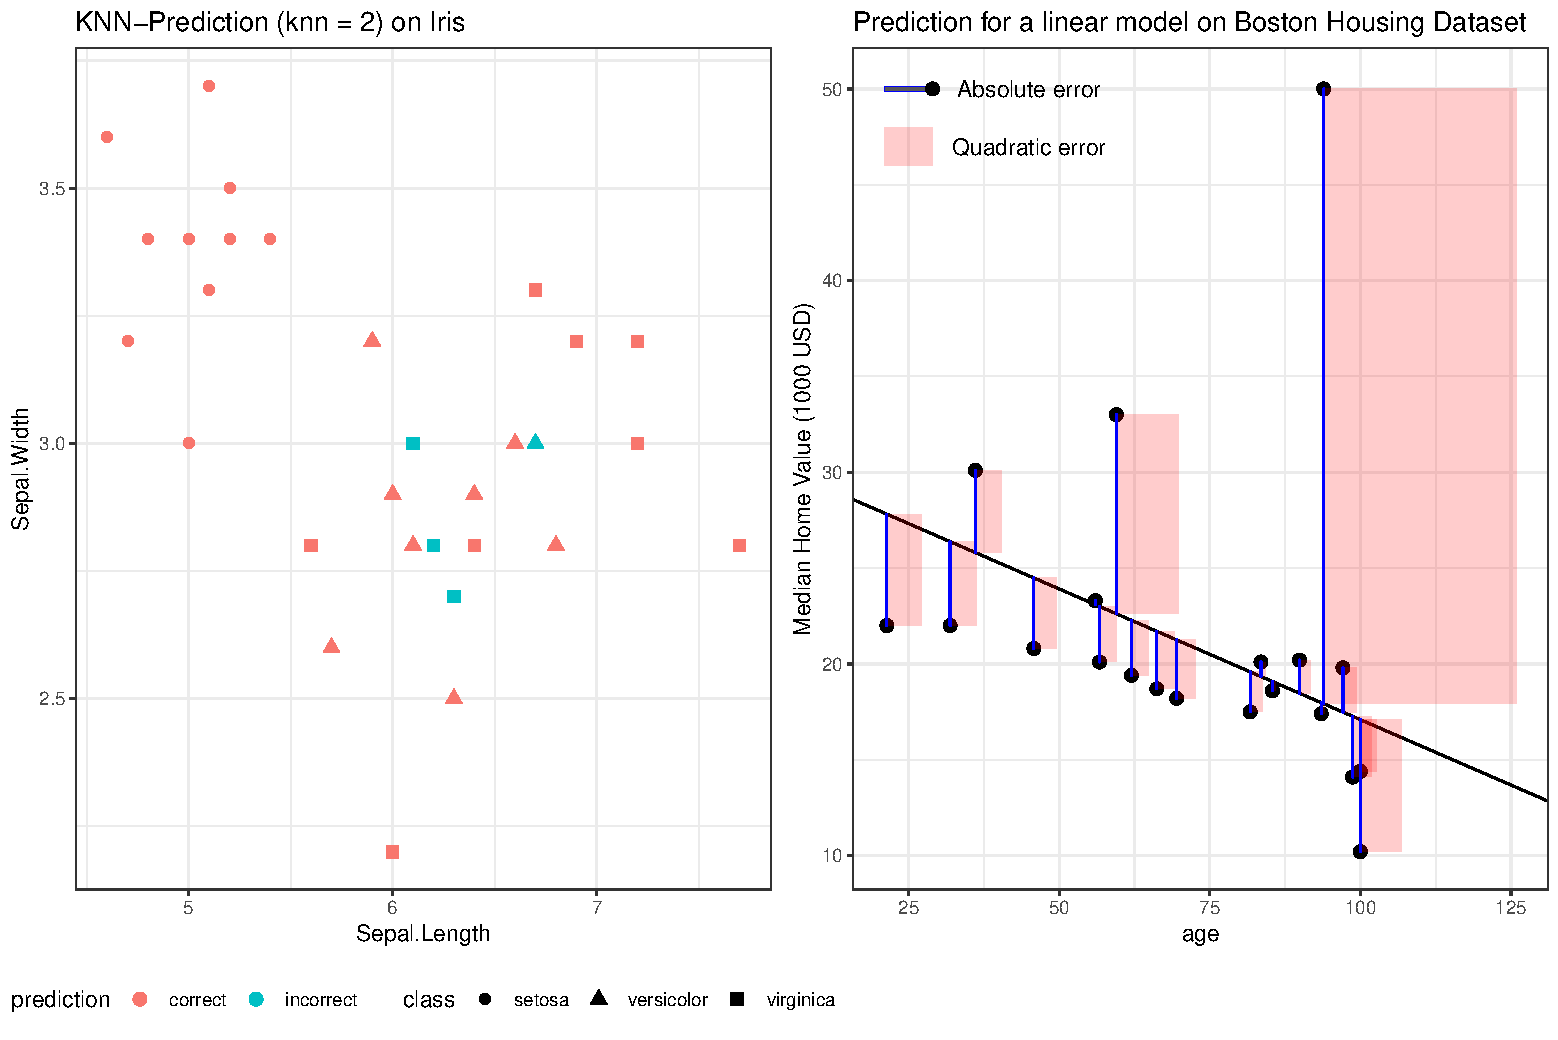
\includegraphics[width=9cm,page=1]{plots/make_classif_regr_error_intro_plot.pdf}
\end{centering}

To compare the performance of two ML models on a single observation or a
new data set, we would ideally like to boil them down to a
\textbf{single} numeric measure of the performance.
\end{frame}


\begin{frame}{Performance Measures vs Loss Functions}
Performance measures are related to losses, but are not the same
\begin{itemize}
\item A performance measure is simply applied at the end, to a fitted model and some test data under consideration. A loss function is optimized by a learning algorithm
\item A performance measure is usually dictated by our prediction problem. There are no technical restrictions on it, except that it needs to be computable and appropriate to evaluate a model on a data set.
A loss function on the other hand needs to be \enquote{handable} by the optimizer (e.g. needs to be differentiabe)
\item Sometimes, performance mearures arer called \enquote{outer losses}, and \enquote{innner loss} is used for the loss minimized by the learner
\item Sometime, one can make the inner loss match the outer loss, so the learning algorithm optimizes exactly the metric we are interested in. But often we use approximations for the inner loss, e.g., for efficiency
\end{itemize}
\end{frame}


\begin{frame}{Performance Measures -Regression:MSE}
The \textbf{Mean Squared Error} compares the mean of the squared
distances between the target variable \(y\) and the predicted target
\(\yh\). \[
MSE = \frac{1}{n} \sumin (\yi - \yih)^2 \in [0;\infty]
\]

Single observations with a large prediction error heavily influence the
\textbf{MSE}, as they enter quadratically

\scriptsize
\begin{center}
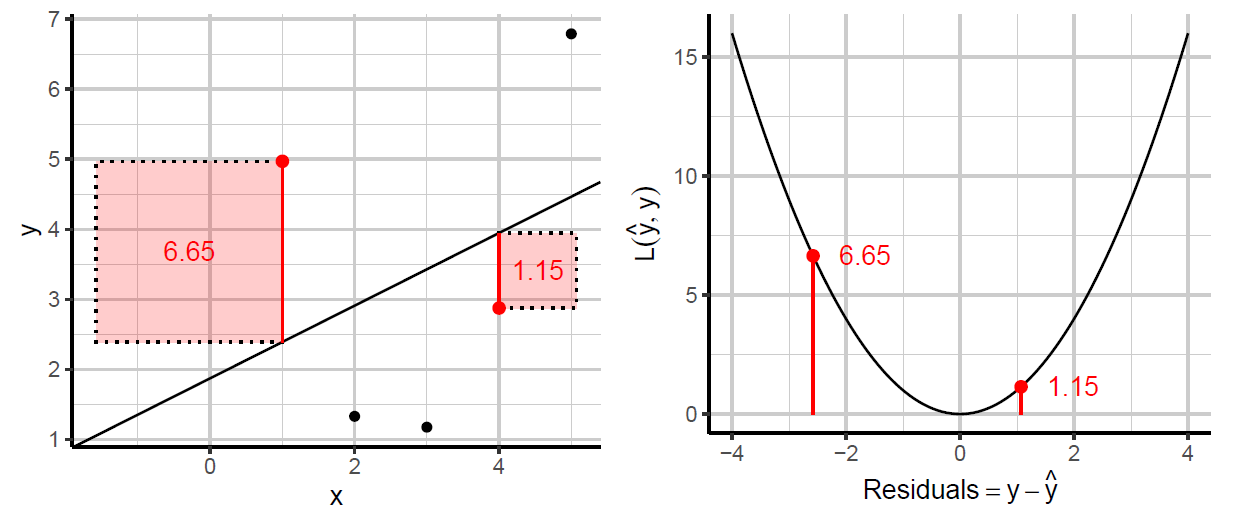
\includegraphics[width=0.9\textwidth]{plots/MSE.png}
\end{center}
\normalsize 
\end{frame}


\begin{frame}{Performance Measures-Regression:MAE}
A more robust (but not neccessarily better) way to compute a performance
measure is the \textbf{Mean Absolute Error}:

\[
MAE = \frac{1}{n} \sumin |\yi - \yih| \in [0;\infty]
\]

The absolute error is more robust. On the other hand, the absolute error
is not differentiable at \(0\).

\scriptsize
\begin{center}
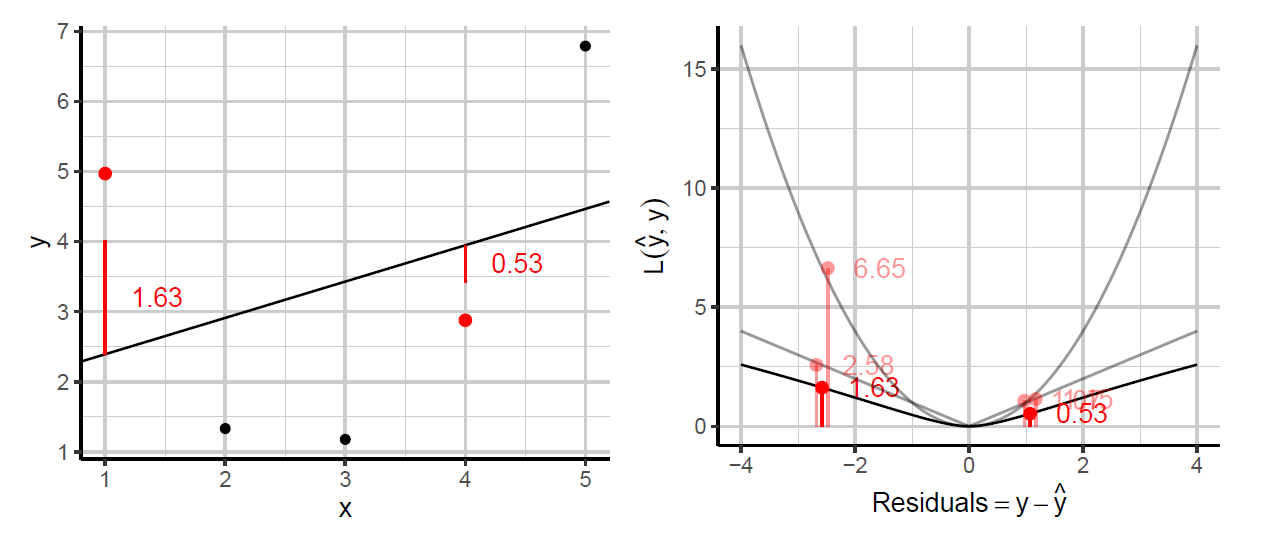
\includegraphics[width=0.9\textwidth]{plots/custom-loss.png}
\end{center}
\normalsize 
\end{frame}


\begin{frame}{Performance Measures - Classification: confusion matrix}
The confusion matrix presents an intuitive way to access the accuracy of a  classification model 
\newline
\begin{centering}
\includegraphics[width=11cm,page=3]{plots/confusion_matrix_measures.pdf}
\end{centering}
\end{frame}



\begin{frame}{Performance Measures - Classification: Accuracy / Error}
The confusion matrix is not a performance measure as such, but most
performance metrics for binary classification are based on it
\newline
\hspace{2cm}\includegraphics[width=11cm,page=4]{plots/confusion_matrix_measures.pdf}

Classification Error = 1 - Accuracy
\end{frame}


\begin{frame}{Performance Measures -Classification: Thresholding}
Thresholding flexibly converts measured probabilities to labels

\begin{centering}
\includegraphics[height=8cm, width=14cm,page=2]{plots/confusion_matrix_measures.pdf}
\end{centering}
\end{frame}


\begin{frame}{Performance Measures-Classification: Overview}
\small
\begin{table}[]
\begin{tabular}{ll}
\hline
\textbf{Classification}& \textbf{Explanation}  \\ \hline
Accuracy              &  Fraction of correct classifications                             \\ \hline
Balanced Accuracy     &  Fraction of correct classifications in each class               \\ \hline
Recall                &  Fraction of positives a classifier captures                     \\ \hline
Precision             &  Fraction of positives in instances predicted as positive        \\ \hline 
F1-Score              &  Tradeoff between precision and recall                           \\ \hline
AUC                   &  Measures calibration of predicted probabilities                 \\ \hline
Brier Score           &  Squared difference between predicted probability                \\ 
                      & and true label                                                   \\ \hline
Logloss               &  Emphasizes errors for predicted probabilities close             \\ 
                      & to 0 and 1                                                       \\ \hline
\end{tabular}
\end{table}
\normalsize

\end{frame}

%%%%%%%%%%%%%%%%%%%%%%%%%%%%%%%%%%%%%%%%%%%%

\section{Generalization}


\begin{frame}{Training Error}
The \textbf{training error} 
is estimated by the average error over the training set
\(\Dtrain\):
\includegraphics[width=10cm,page=4]{plots/train_error.png}

It is usually a very unreliable and overly optimistic estimator of future performance (e.g. training 1-NN is always zero).
\end{frame}


\begin{frame}{Example: Polynomial Regression}
Assume we have a single, univariate \(x\) and that \(y\) can be
approximated by a \(d\)th-order polynomial

\[ \fxt = \theta_0 + \theta_1 x + \cdots + \theta_d x^d = \sum_{j = 0}^{d} \theta_j x^j\text{.} \]

\(\theta_j\) are the coefficients and \(d\) is called the degree.

This is still linear regression / a linear model, and for a fixed \(d\),
the \(\theta\) can easily be obtained through the normal equations.
\end{frame}



\begin{frame}{Example: Polynomial Regression}
True relationship is
\(f(x) = 0.5 + 0.4 \cdot \sin (2 \pi x) + \epsilon\)

\scriptsize

\begin{center}
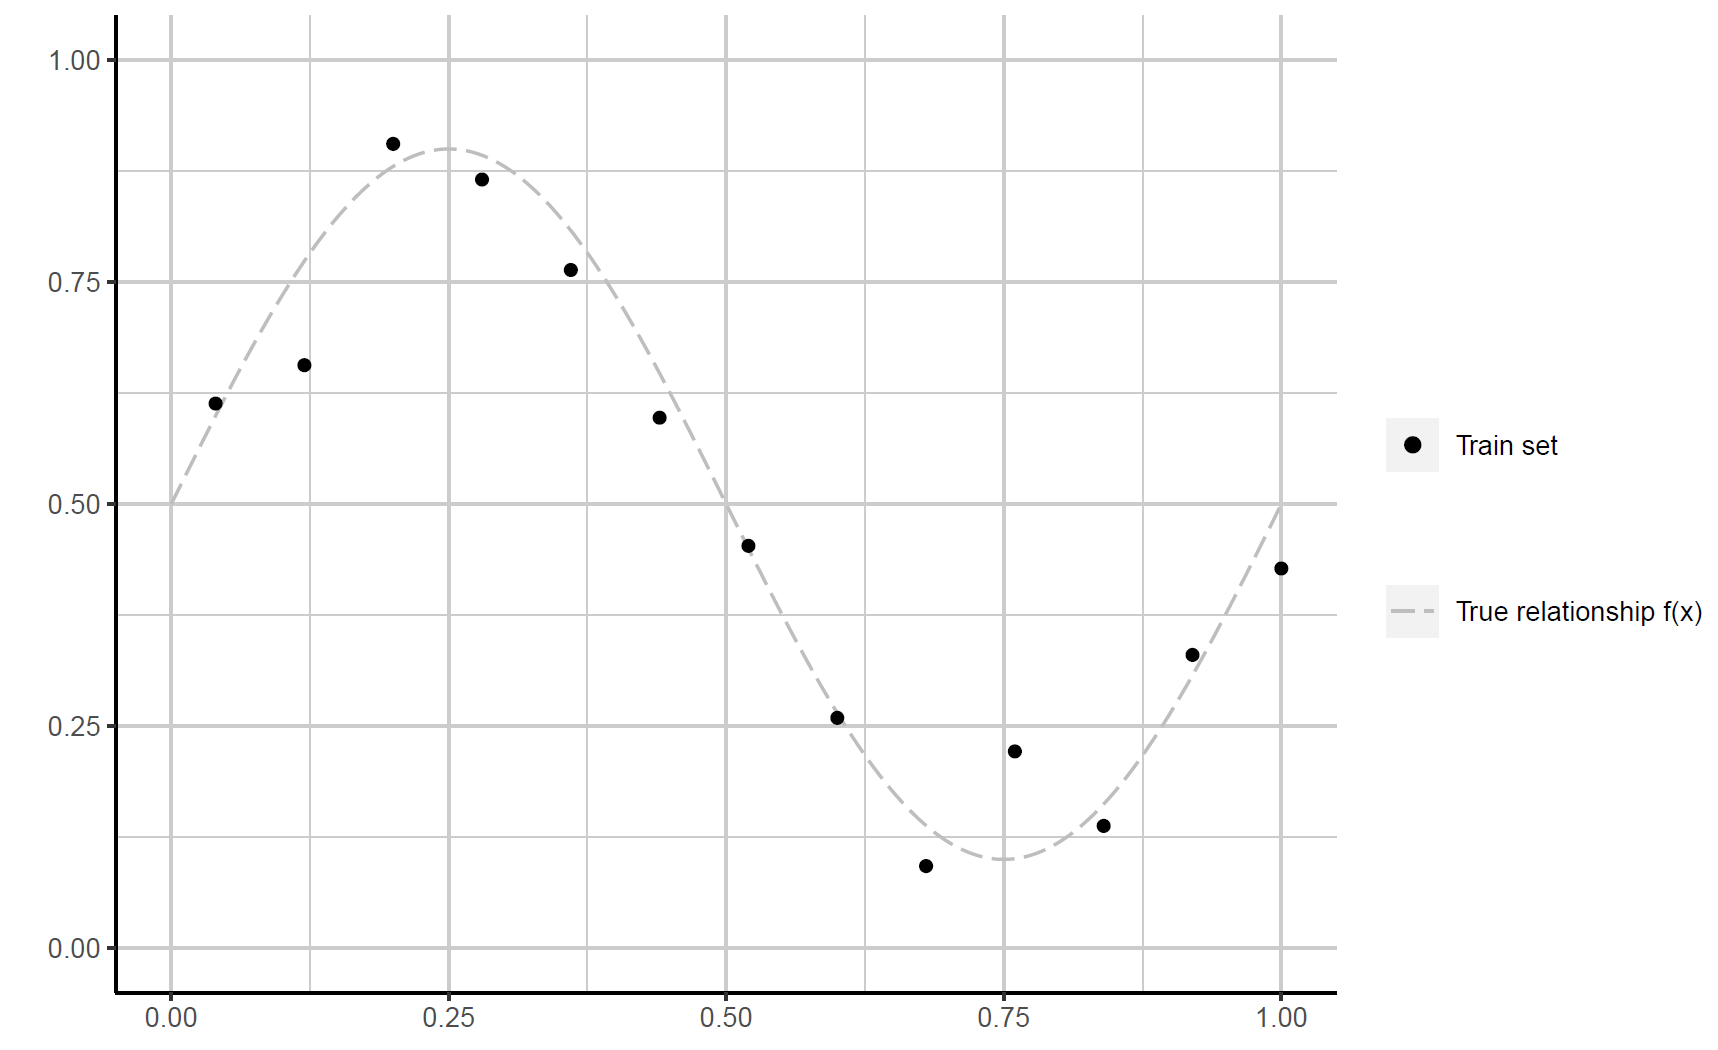
\includegraphics[width=0.9\textwidth]{plots/poly-reg01.png}
\end{center}

\normalsize 
\end{frame}


\begin{frame}{Example: Polynomial Regression}
Models of different \textbf{complexity}, i.e., of different orders of the
polynomial, are fitted. How should we choose \(d\)?

\scriptsize

\begin{center}
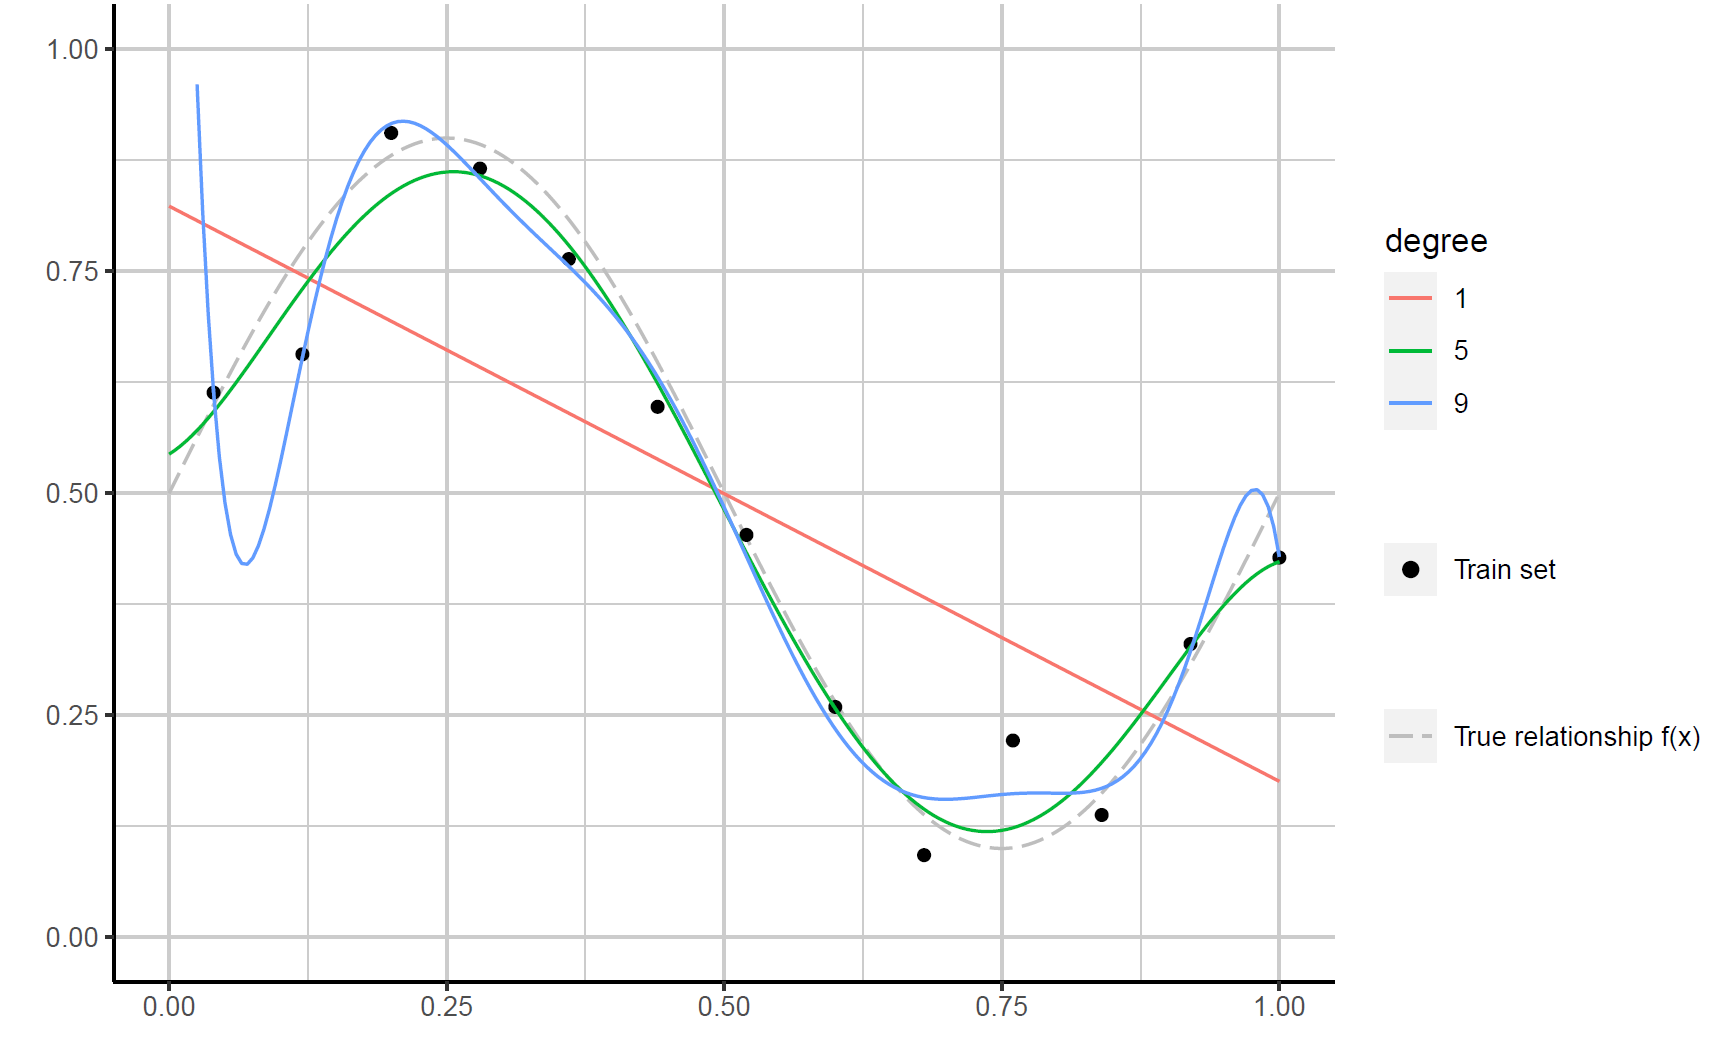
\includegraphics[width=0.9\textwidth]{plots/poly-reg02.png}
\end{center}
\normalsize 
\end{frame}


\begin{frame}{Example: Polynomial regression}
The performance of the models on the training data can be measured by
calculating the training error according to the mean squared
error (MSE) criterion:

\[ \frac{1}{n} \sum_{i = 1}^{n}(y_i - \hat{y}_i)^2\text{.} \]

d = 1: 0.03, \qquad d = 5: 0.002, \qquad d = 9: 0.001 \\

\vfill
Observation: Simply using the training error for model evaluation seems to be a bad idea!
\end{frame}


\begin{frame}{Test Error and Hold-Out Splitting}
Problem: How to estimate the generalization error, i.e. the prediction error for  \enquote{new unseen data}?

Solution: Hold-out splitting and evaluation

\begin{itemize}
\item Straightforward idea:
 measure performance on a new set of data not used during training
\item For a given set \(\D\), we have to preserve some data for testing that
  we cannot use for training. We need to define a training set \(\Dtrain\) and a test set \(\Dtest\), e.g.~by randomly partitioning the original dataset \(\D\)
\end{itemize}
\end{frame}


\begin{frame}{Test Error and Hold-Out Splitting}
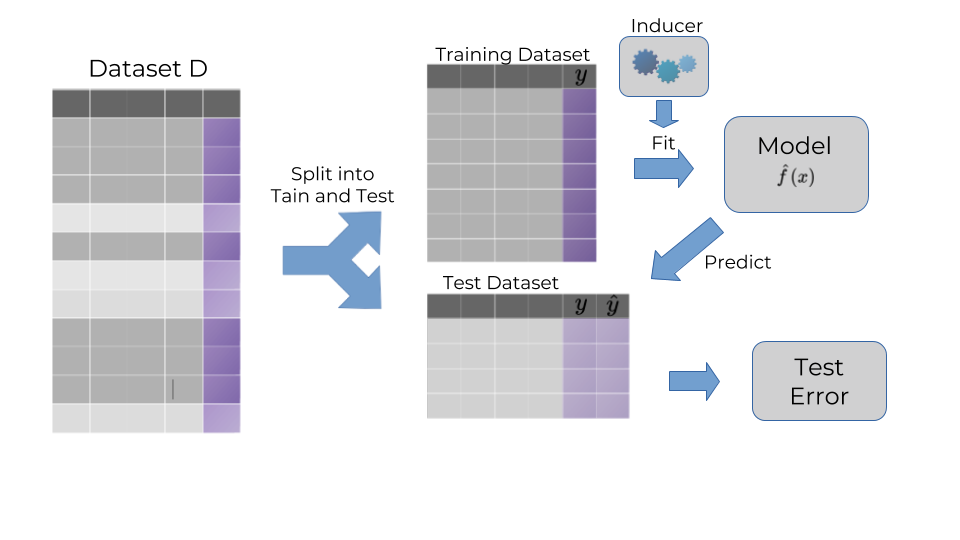
\includegraphics[width=11cm]{plots/test_error.png}
\end{frame}


\begin{frame}{Example: Polynomial Regression}
\scriptsize

\begin{center}
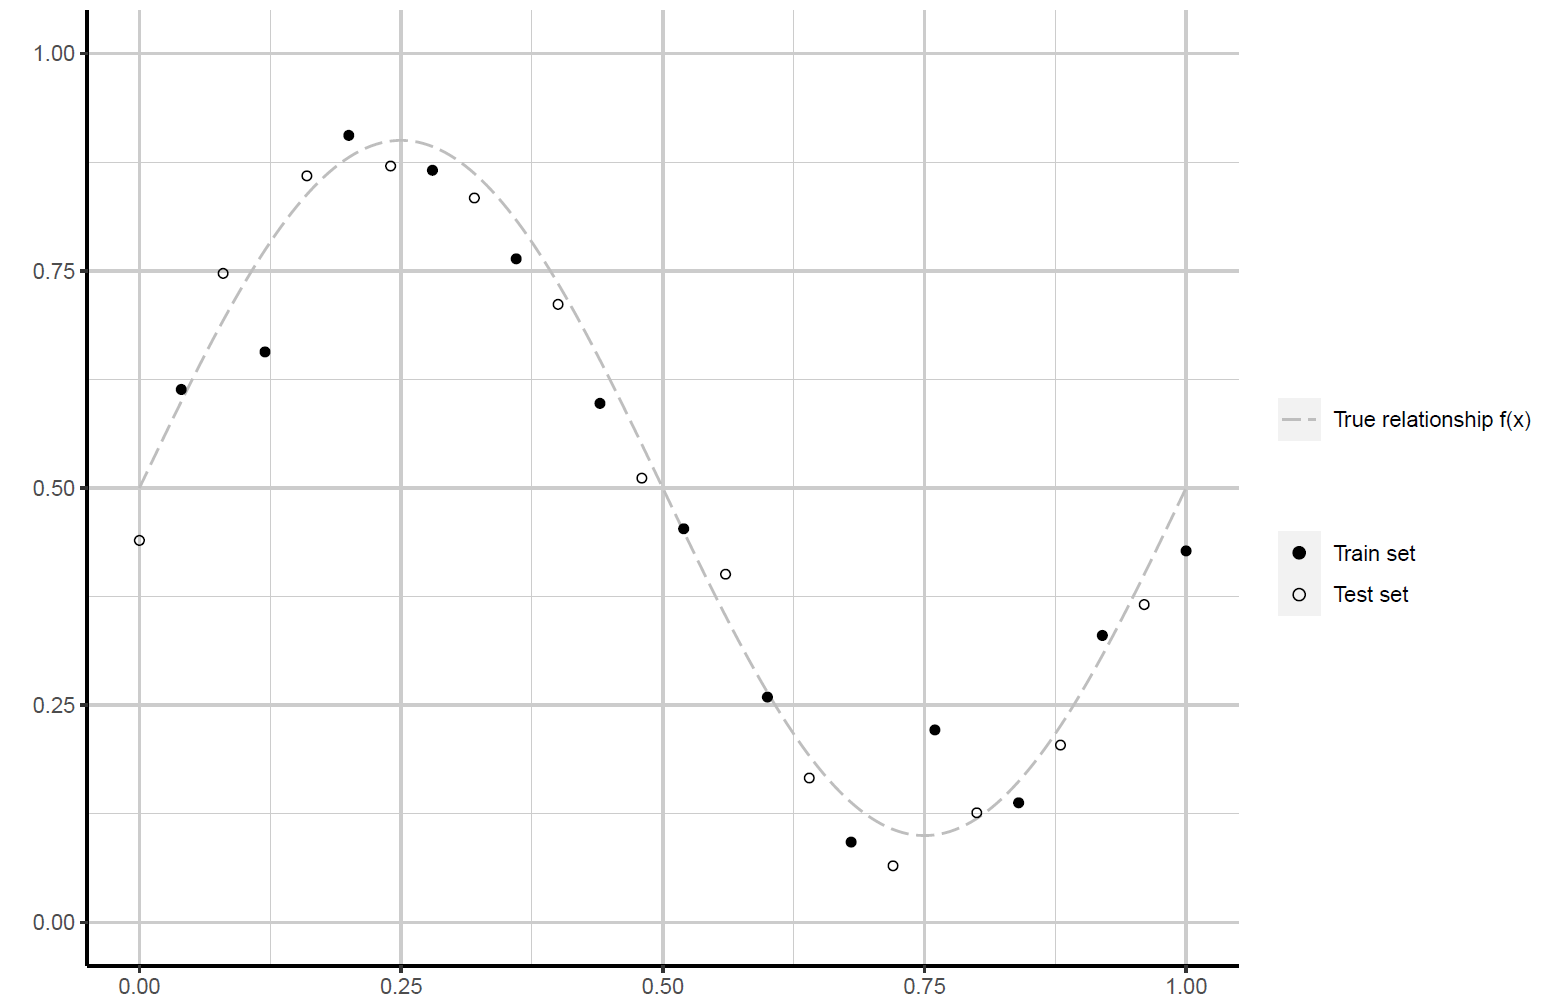
\includegraphics[width=0.9\textwidth]{plots/test_error01.png}
\end{center}

\normalsize 
\end{frame}


\begin{frame}{Example: Polynomial Regression}
\scriptsize

\begin{center}
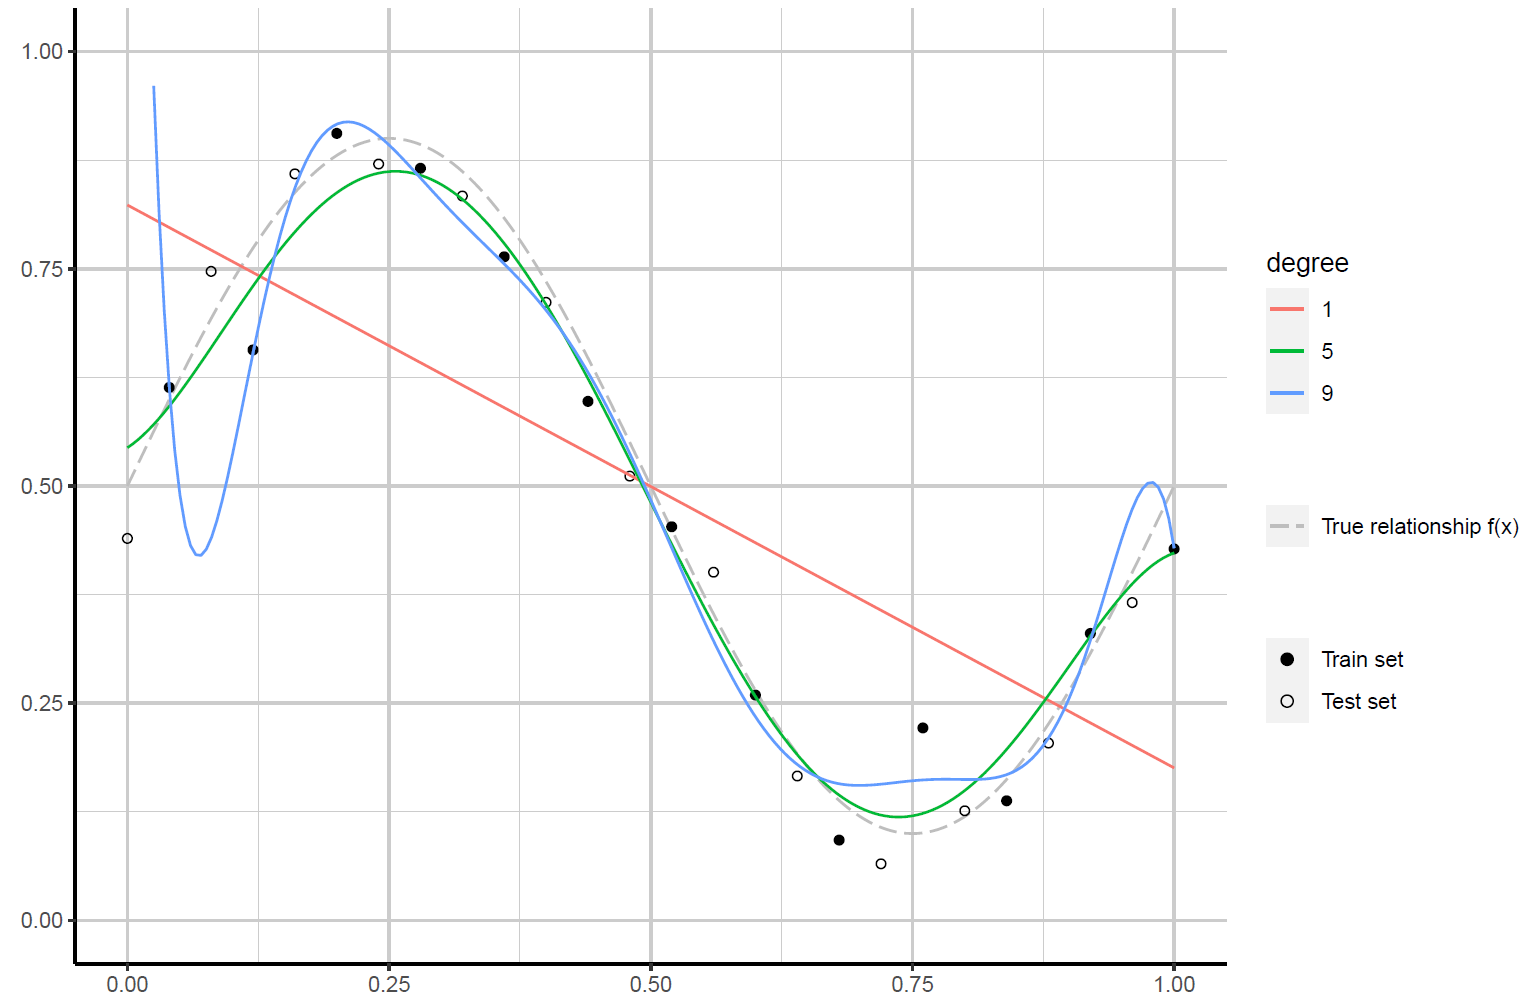
\includegraphics[width=0.9\textwidth]{plots/test_error02.png}
\end{center}

\normalsize 
\end{frame}


\begin{frame}{Test Error and Hold-Out Splitting}
\scriptsize

\begin{center}
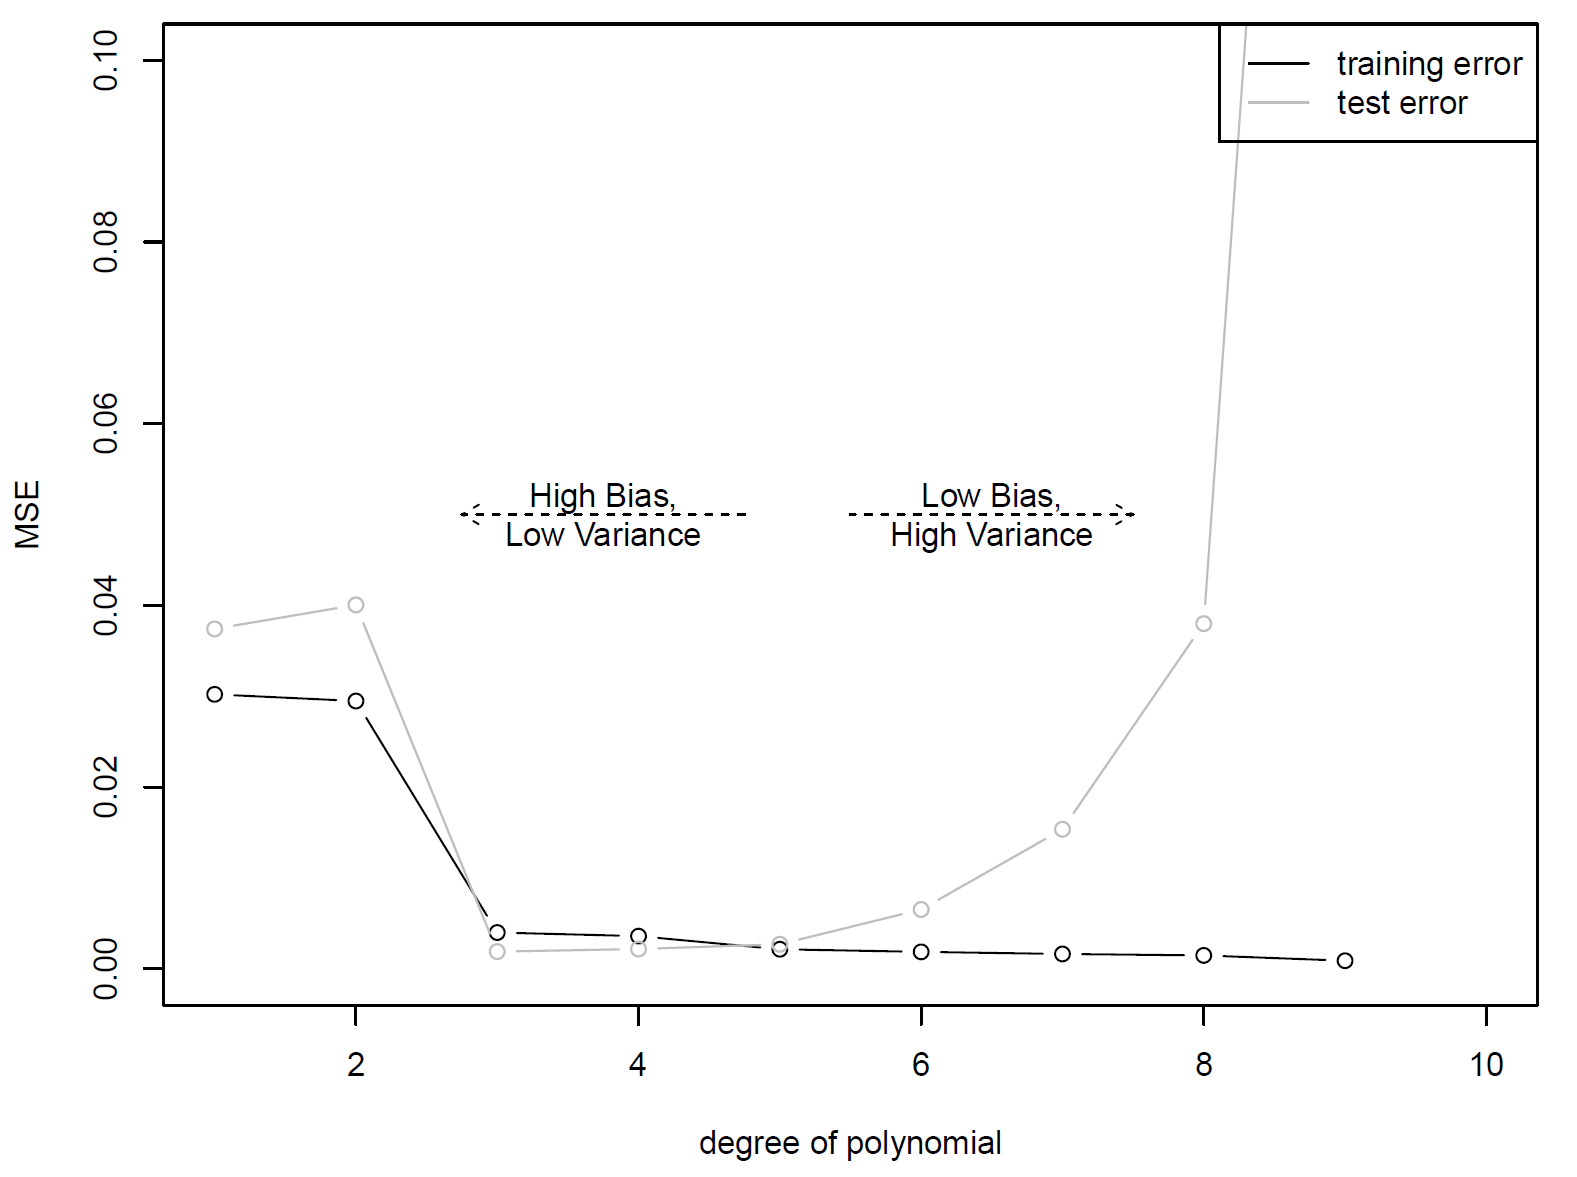
\includegraphics[width=0.8\textwidth]{plots/test_error03.png}
\end{center}

\normalsize  Test error is best for \(d=3\)
\end{frame}


\begin{frame}{Training vs.~Test Error}
The training error

\begin{itemize}
\item is an over-optimistic, biased estimator as the performance is
  measured on the same data the  model  was trained on
\item decreases with smaller training set size as it is easier for the model
  to learn the underlying structure in the training set perfectly
\item decreases with increasing model complexity as the model is able to
  learn more complex structures
\end{itemize}

The test error

\begin{itemize}
\item will typically decrease when the training set increases as the model
  generalizes better with more data
\item will have higher variance with decreasing test set size
\item will have higher variance with increasing model complexity
\end{itemize}

\end{frame}



\begin{frame}{Resampling}
\begin{itemize}
\item  If $\D$ is not huge, we need to construct a performance estimator that uses the data more efficiently
\item \textbf{Resampling}: split the data set repeatedly into training and tests sets, and aggregate (e.g.~average) the results
\item The usual trick is to make training sets larger (to keep the bias small), and to handle the variance introduced by smaller test sets through many repetitions and averaging of results.
\end{itemize}
\end{frame}

\begin{frame}{Resampling}
\begin{itemize}
\item Aim: estimate the actual model performance.
\item Uses the data more efficiently than a simple train-test split.
\item Repeatedly split in train and test, then aggregate results.
\end{itemize}

\begin{center}
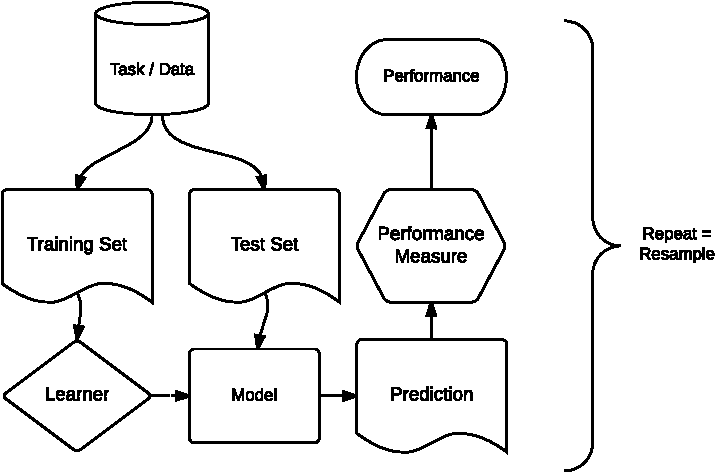
\includegraphics[width=7cm]{plots/ml_abstraction-crop.pdf}
\end{center}
\end{frame}



\begin{frame}{Cross-Validation}
\begin{itemize}
\item Split the data into \(k\) roughly equally-sized partitions
\item Use each part once as test set and joint \(k-1\) others as training set
\item Obtain \(k\) test errors and average
\end{itemize}

Example: 3-fold cross-validation:

\begin{center}
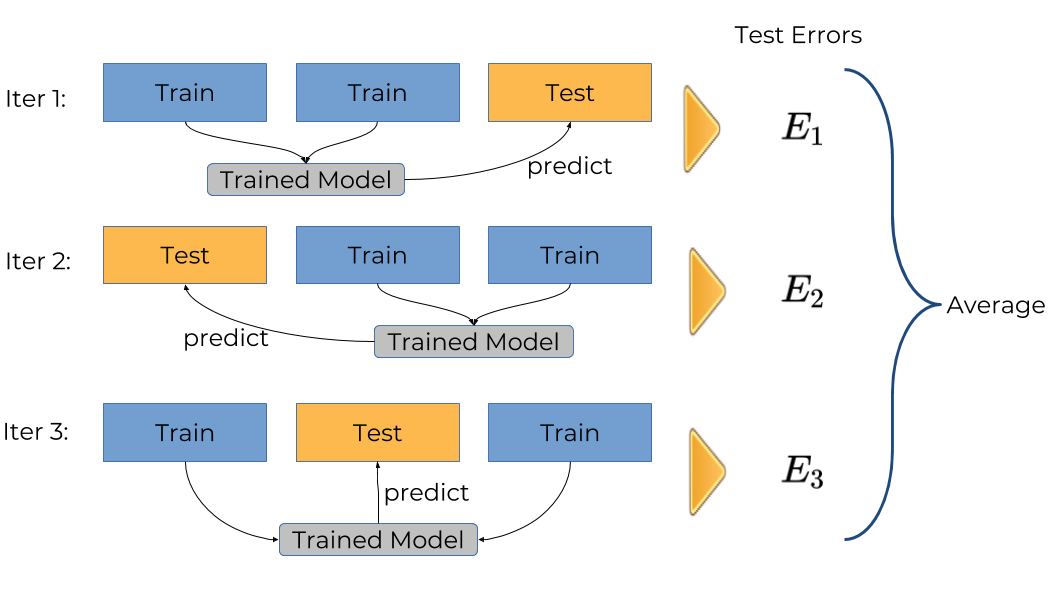
\includegraphics[width=7cm]{plots/crossvalidation.png}
\end{center}
\end{frame}


\begin{frame}{Cross-Validation}
\begin{itemize}
\item \(k = n\) is known as \textbf{leave-one-out (LOO)} cross-validation or
  jackknife.
\item The performance estimates for each fold are NOT independent, because
  of the structured overlap of the training sets. 
\item LOO is  a nearly unbiased estimator for the performance after training on the full data set, but has high variance.
\item Repeated \(k\)-fold CV (multiple random partitions) can improve error
  estimation for small sample size.
\end{itemize}
\end{frame}


\begin{frame}{Summary: Training/evaluating a learning algorithm with limited data}

\begin{itemize}
\item If data is limited, one wants to use all available data for training
\item Problem: we need to estimate how well 
  the learning algorithm performs in the future,
  but no data 
  is left to reliably do this

\item Idea: approximate how well the learner works when it sees nearly \(n\) points from the same data distribution.
\item Use holdout splittung/ CV/resampling to produce performance estimates. When using much less data in fitting than \(n\), we \enquote{hurt} the learner unfairly (pessimistic bias)
\item This is done to estimate the performace, not to produce models, parameters, etc. These are intermediate results and discarded
\item The model and final parameters are obtained by training on the complete dataset. 
\end{itemize}
\end{frame}

%%%%%%%%%%%%%%%%%%%%%%%%%%%%%%%%%%%%%%%%

\section{Overfitting and Regularization}

\begin{frame}{Overfitting to training data}
\begin{itemize}
\item Learner finds a pattern in the data that is not actually true in the real world, it \textbf{overfits} the data
\item Every powerful learner can \enquote{hallucinate} patterns
\item Happens when you have too many hypotheses and not enough data to tell them apart
\item The more data, the more \enquote{bad} hypotheses are eliminated
\item If the hypothesis space is not constrained, there may never be enough data
\item There is often a parameter that allows you to constrain (\textbf{regularize}) the learner
\end{itemize}
\end{frame}


\begin{frame}{Overfitting to training data}

\begin{center}
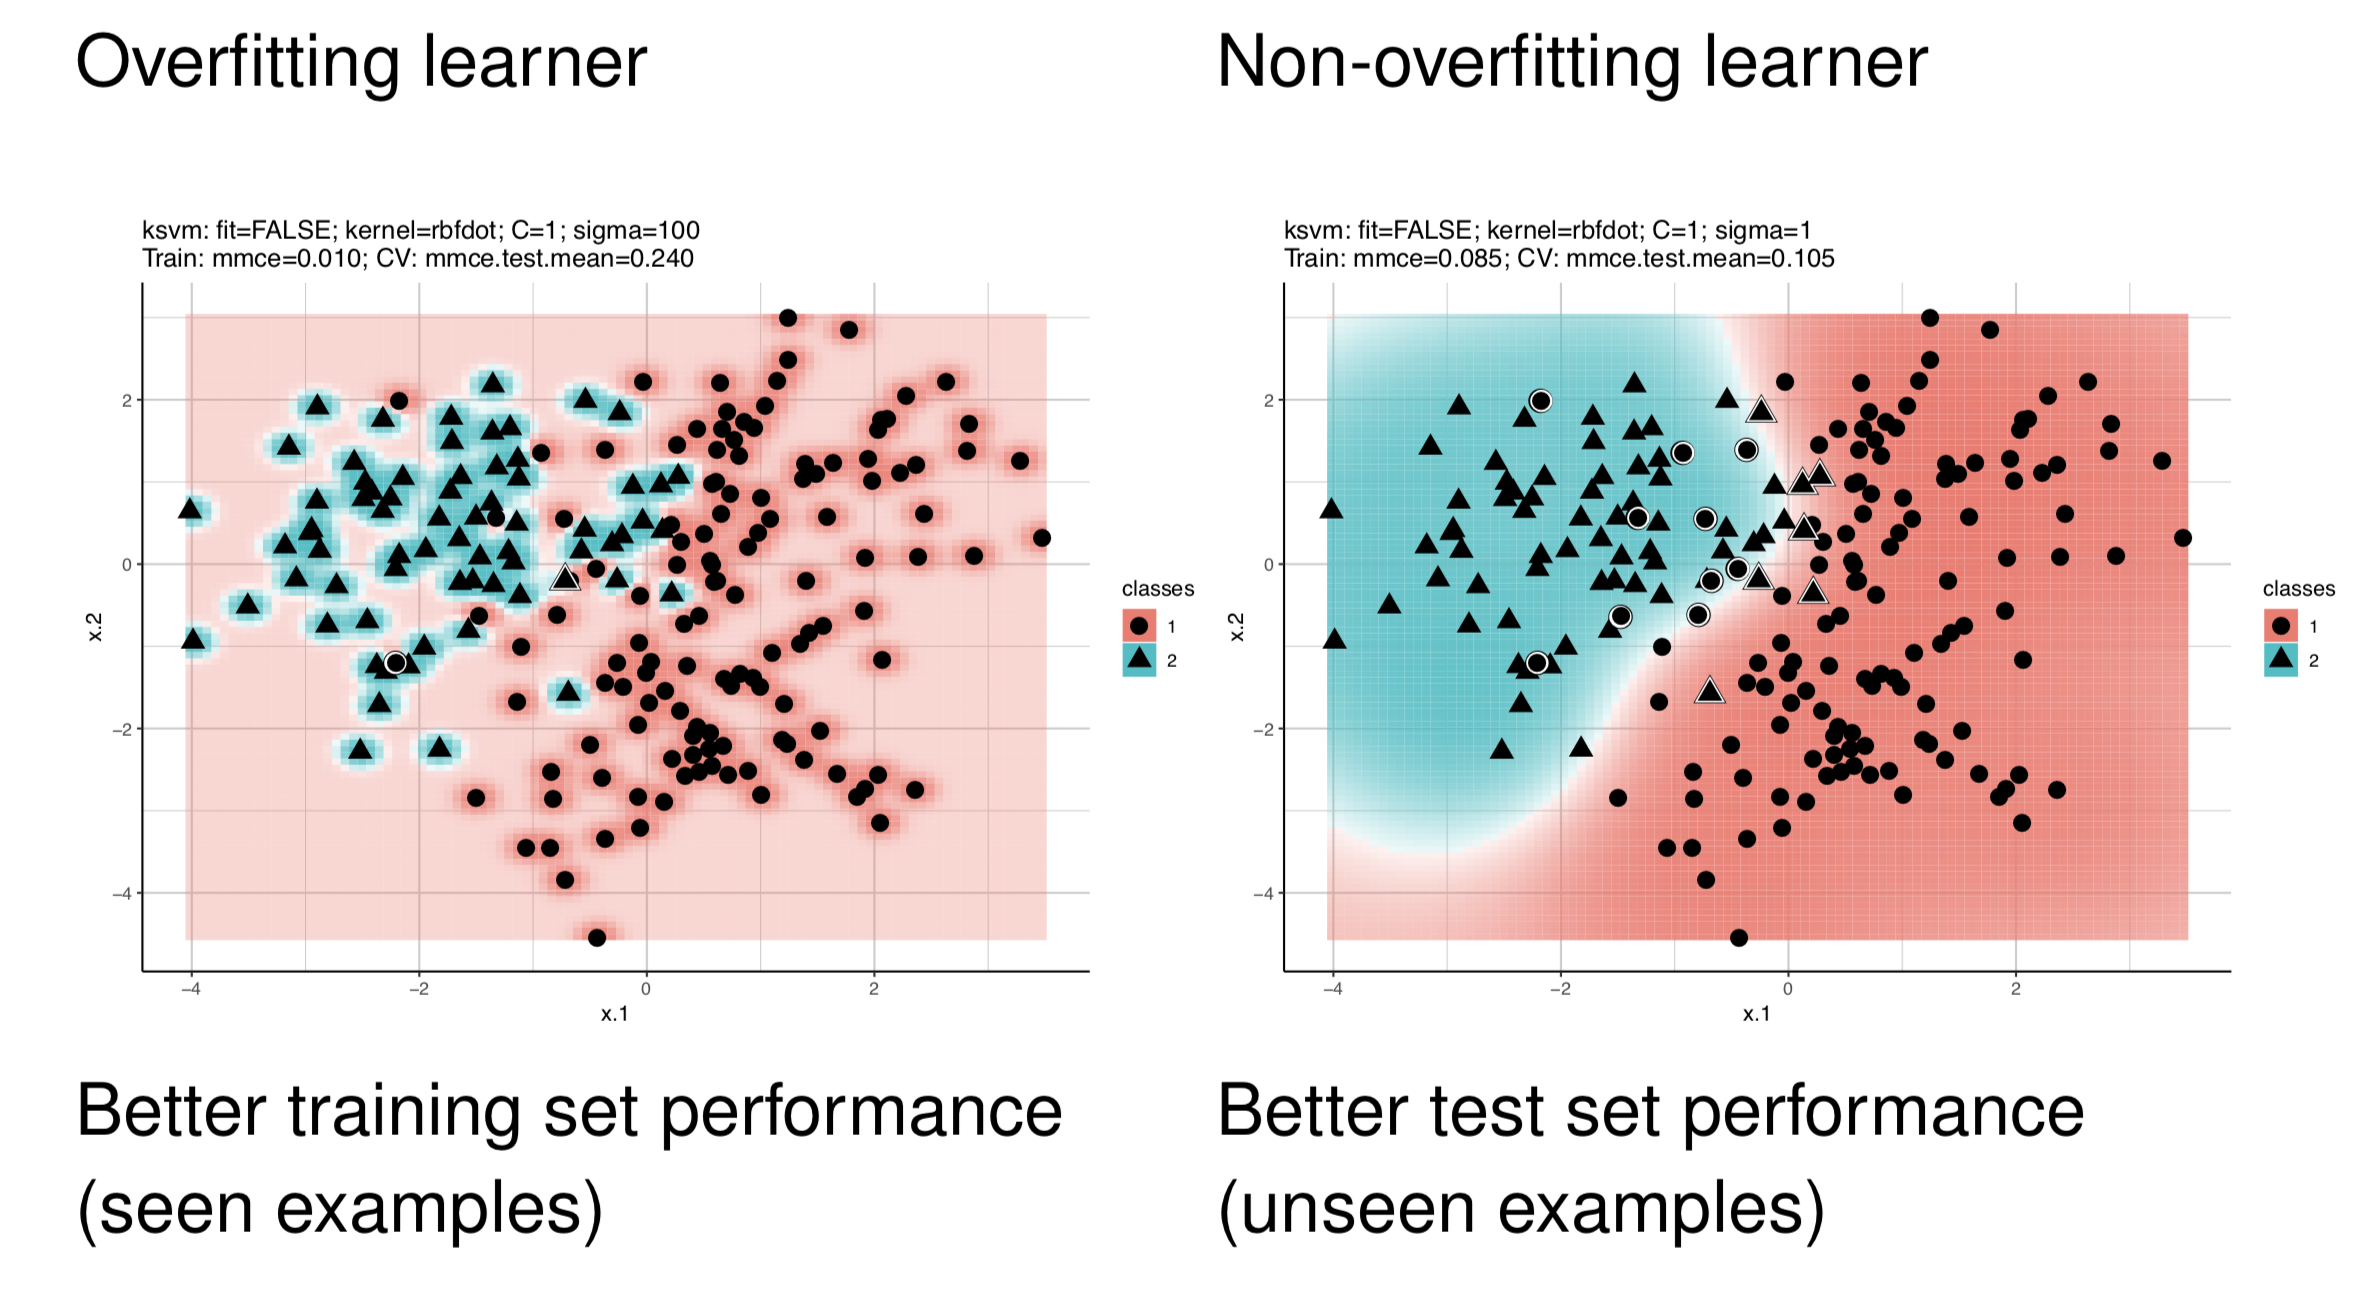
\includegraphics[width=12cm]{plots/overfitting.png}
\end{center}
\end{frame}


\begin{frame}{Overfitting and Noise}
\begin{itemize}
\item Overfitting is seriously exacerbated by \emph{noise} (errors in the training data)
\item An unconstrained learner will start to model that noise
\item It can also arise when relevant features are missing in the data
\item In general it's better to make some mistakes on training data (\enquote{ignore some observations}) than trying to get all correct
\end{itemize}
\end{frame}


\begin{frame}{Triple Trade-Off}
When learning a model from data, there is a trade-off between three factors:

\begin{itemize}
\item complexity of the hypothesis space 
\item amount of training data (in terms of both instances and informative features)
\item generalization error on new examples
\end{itemize}

\vfill

If the complexity of the hypothesis space is large enough to approximate the data generating process, the generalization error will decrease as the amount of training data increases. 
\end{frame}


\begin{frame}{Trade-Off Between Generalization Error and Complexity}
For a fixed ammount of training data, the generalization error (i.e. actual error) decreases first and then starts to increase (overfitting) as the complexity of the
hypothesis space \(H\) increases.

\scriptsize
\begin{center}
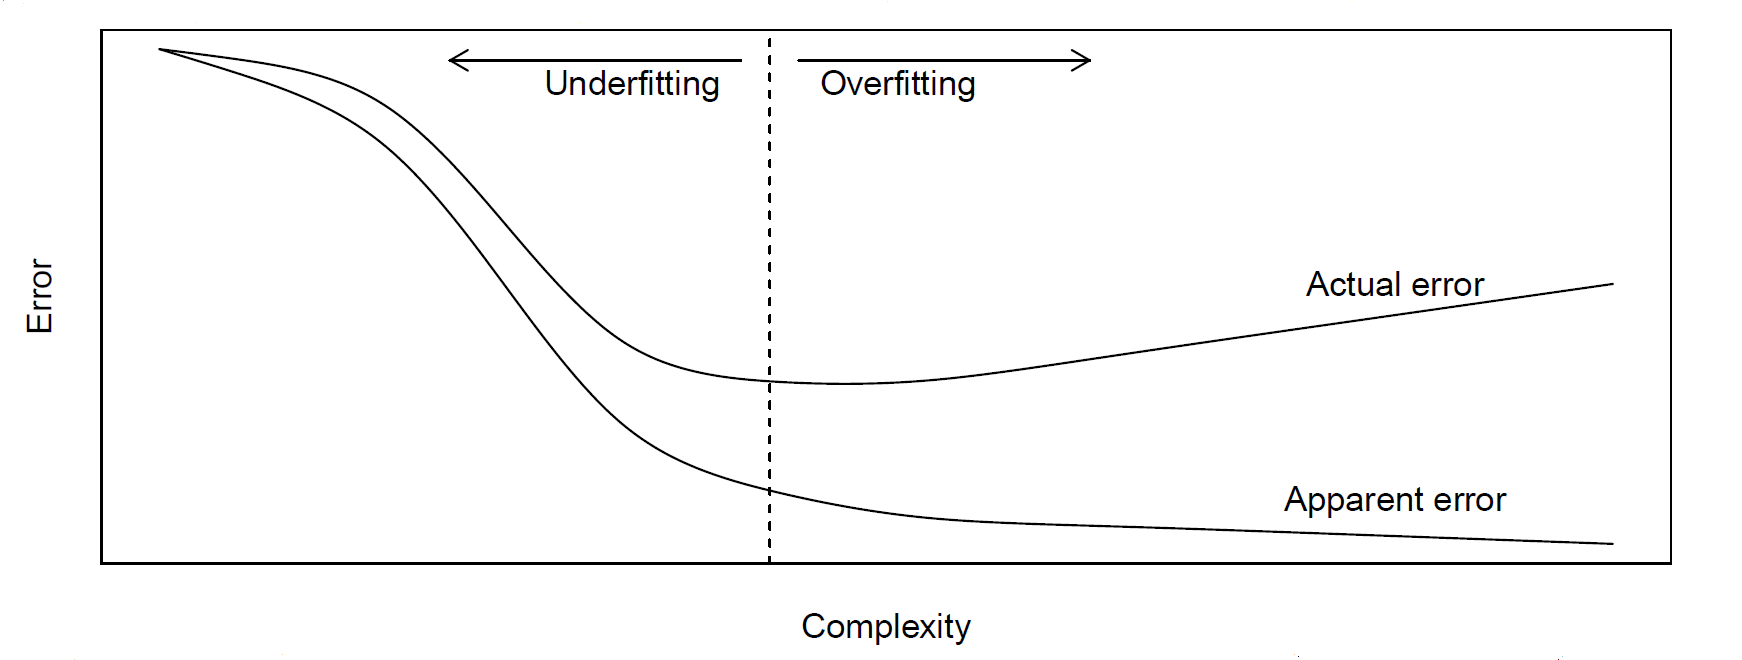
\includegraphics[width=0.9\textwidth]{plots/trade-off.png}
\end{center}

\normalsize  \vspace{-0.2cm} \(\Rightarrow\) 
Goal: Find the "right" amount of complexity for the given amount of data where generalization error becomes minimal.
\end{frame}


\begin{vbframe}{How to avoid Overfitting}
Why can \textbf{overfitting} happen? And how to avoid it?
\begin{itemize}
\def\labelenumi{\arabic{enumi}.}
\item Not enough data \(\to\) collect \textbf{more data}
\item Data is noisy \(\to\) collect \textbf{better data} (reduce noise) 
\item Aggressive loss optimization \(\to\) \textbf{optimize less}
\item Models are too complex \(\to\) use \textbf{less complex models}
\end{itemize}

Mechanisms to avoid overfitting are often reffered to as \textbf{regularization}.
\end{vbframe}


\begin{vbframe}{Overfitting: Example}

Assume we want to predict the daily maximum \textbf{ozone level} in LA
given a data set containing \(50\) observations.

\vfill

We use (a subset of) the \texttt{Ozone} data set from the \texttt{mlbench} package:
It contains \(12\) features describing time conditions (e.g., weekday, month), the weather (e.g.~temperature at different weather stations, humidity, wind speed) or geographic variables (e.g.~the pressure gradient).

\framebreak

We fit a linear regression model using \emph{all} of the features

\[
f(x | \theta) = \theta^Tx = \theta_0 + \theta_1 x_1 + \theta_2 x_2 + ... + \theta_{12} x_{12}.
\]

We evaluate the performance with \(10\) times \(10\)-fold CV.

\vfill

While our model fits the training data almost perfectly (left), it generalizes poorly to new test data (right). We \textbf{overfitted}.

\begin{center}
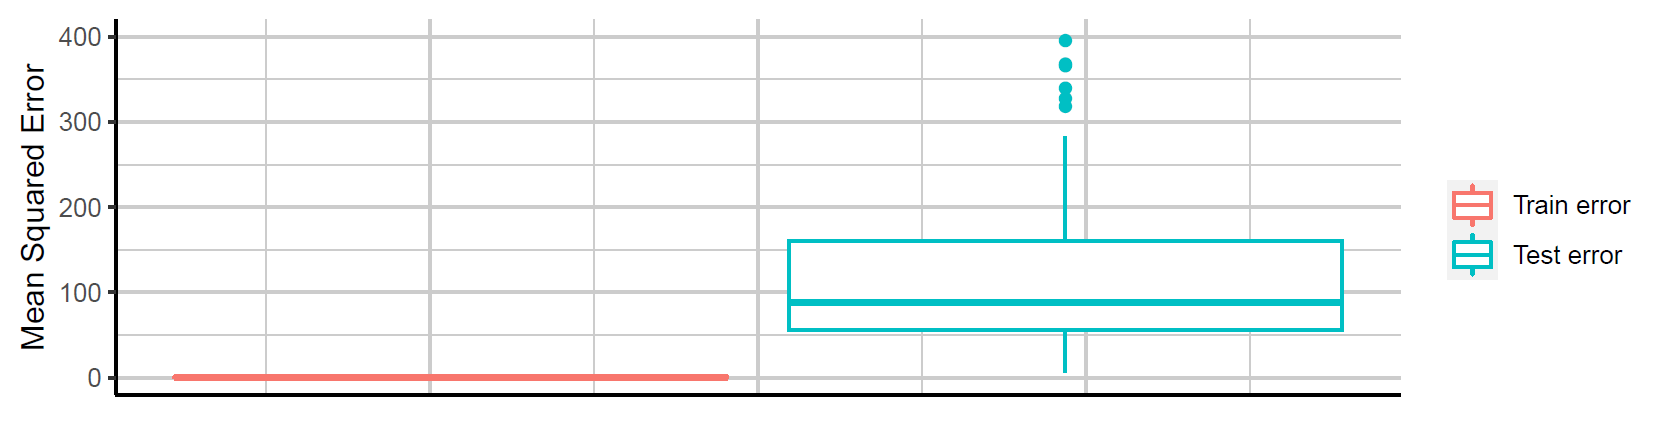
\includegraphics[width=0.9\textwidth]{plots/regularization.png}
\end{center}

\end{vbframe}


\begin{vbframe}{How to avoid Overfitting}
\textbf{Approach 1: collect more data}
Example: We explore our results for increased data set size by \(10\) times
\(10\)-fold CV. The fit worsens slightly, but the test error decreases.

\vfill

\begin{center}
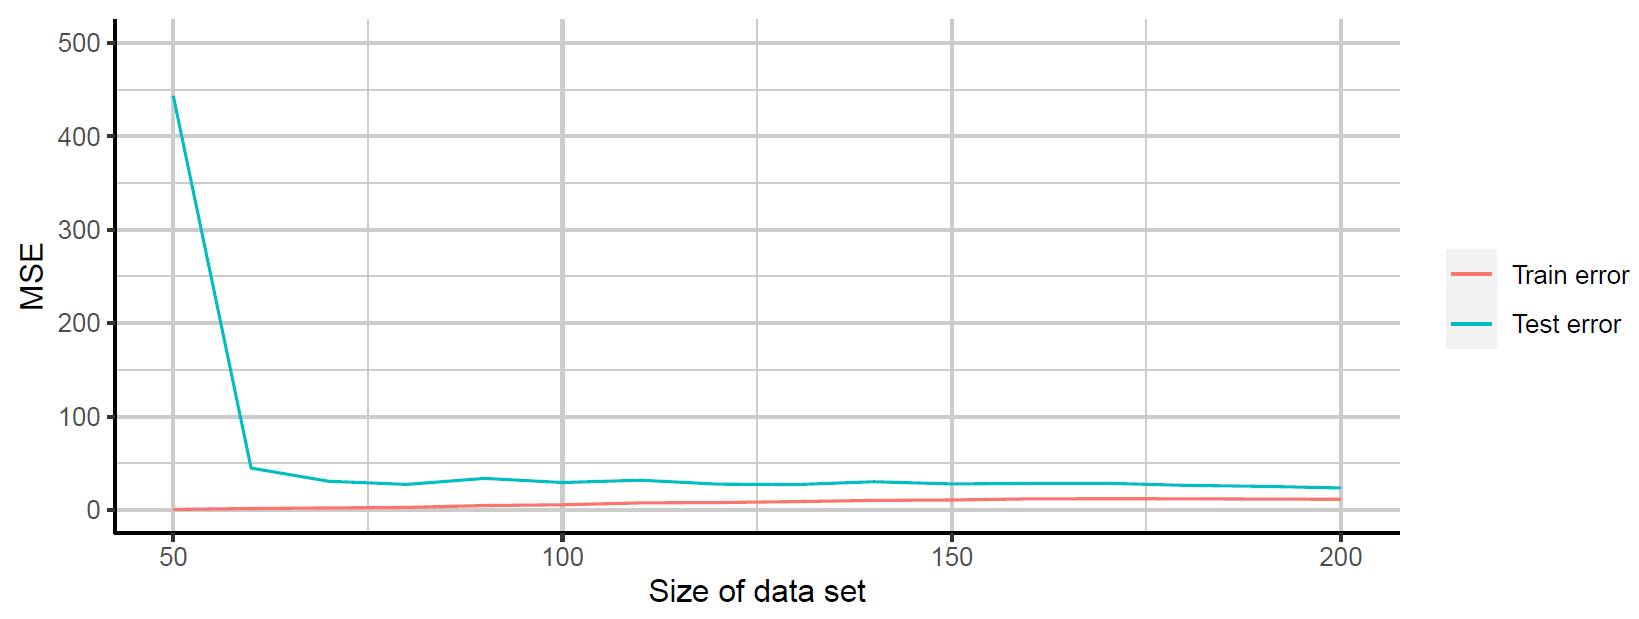
\includegraphics[width=0.9\textwidth]{plots/regularization02.png}
\end{center}

Good idea, but often not feasible in practice.

\framebreak

\textbf{Approach 2}: \textbf{early stopping}
When performing iterative optimization, display model performance on an hold out \\\textbf{validation set} (final performance still needs to evaluated on a test set!).

\begin{center}
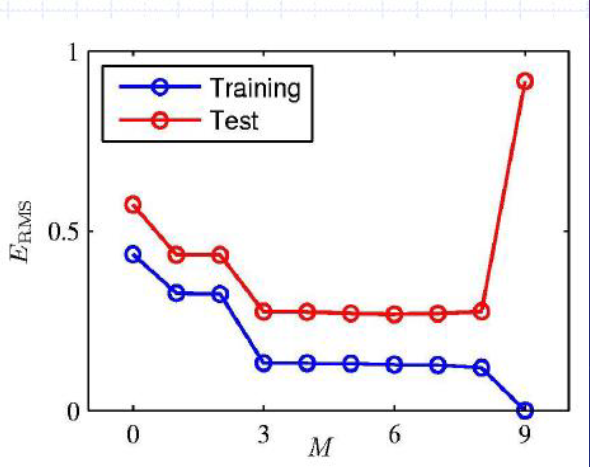
\includegraphics[width=7cm]{plots/early_stopping.png}
\end{center}

\framebreak

\textbf{Approach 3}: reduce \textbf{complexity}

Example: 
To model the ozone level:
\begin{itemize}
\item we try the simplest model we can think of: we dont use any features, but always predict the empirical mean (i.e. intercept only model/ featureless predictor)

\[
f(x | \theta) = \theta_0 = \frac{1}{n}\sumin \yi
\]

\item 
We then increase the complexity of the model step-by-step by adding one
feature at a time.

\end{itemize} 

\framebreak

We can control the complexity of the model by including/excluding
features. We can try out all feature combinations and investigate the
model fit.

\vfill

\begin{center}
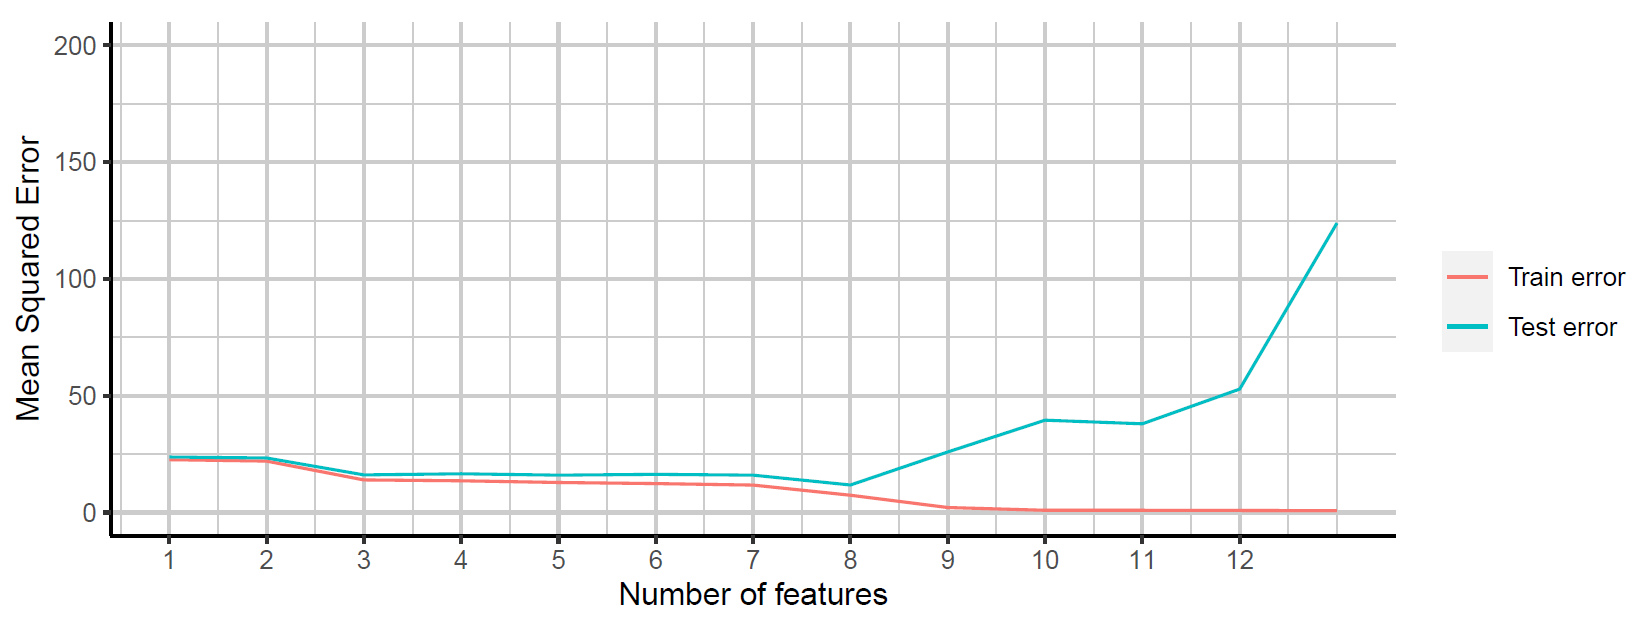
\includegraphics[width=0.9\textwidth]{plots/regularization03.png}
\end{center}

Note: For simplicity, we added the features in one specific order - but there are $2^{12} = 4096$ potential feature combinations.
\end{vbframe}


\begin{vbframe}{Regularization: Complexity vs.~Fit}
We have have contradictory goals
\begin{itemize}
\item \textbf{maximizing the fit} (minimize the train loss)
\item \textbf{minimizing the complexity} of the model.
\end{itemize}

We need to find the \enquote{sweet spot}.

\begin{center}
\begin{figure}
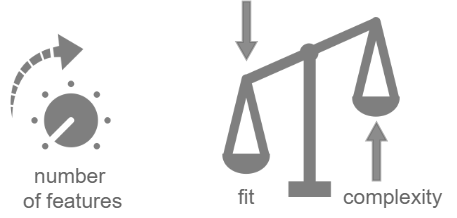
\includegraphics[width=0.6\textwidth]{plots/complexity-vs-fit.png}
\end{figure}
\end{center}

\framebreak

We saw that we can control model complexity by adding/removing features. 

\vfill 

Instead of controlling the complexity in a discrete way (e.g. by specifying
the features), we might prefer to control the complexity
\textbf{on a continuum} from simple to complex.

\vfill

\begin{center}
\begin{figure}
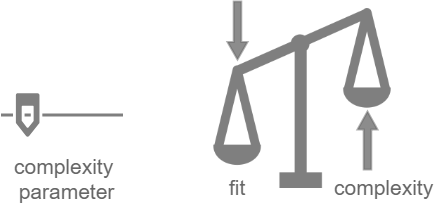
\includegraphics[width=0.6\textwidth]{plots/complexity-vs-fit-continuous.png}
\end{figure}
\end{center}

\end{vbframe}


\begin{frame}{Regularized Linear Regression}
Instead of pure \textbf{empirical risk minimization}, we add a penalty
for complex (read: large) parameters \(\theta_j\):

\[
\riskrt = \sumin \left(\yi - \theta^T \xi\right)^2 + \lambda \cdot \underbrace{J(\theta)}_{\text{penalty}}
\]

\begin{itemize}
\item The parameter \(\lambda\) is called \textbf{regularization (hyper)parameter}, it controls the complexity of the learned model  
\item If \(\lambda = 0\), \(\riskrt\) reduces to simple empirical risk minimization
\end{itemize}

\end{frame}


\begin{frame}{Ridge Regression}
If we choose \(J(\theta)\) to be the \(L_2\)-penalty\(^{(*)}\), the
model is called \textbf{ridge regression}.
It tries to \emph{shrink} the regression coefficients \(\theta\) towards
\(0\). We minimize:
\vspace{-0.3cm}
\[
\mathcal{R}_{ridge}(\theta) = \sumin (\yi - \theta^T \xi)^2 + \lambda ||\theta||_2^2
\]

\pause

$^{(*)}$ The $L_2$ norm or Euclidean norm is $||\theta||_2^2 = \theta_1^2 + \theta_2^2 + ... + \theta_p^2$
\vspace{-0.3cm}
\begin{figure}
\center
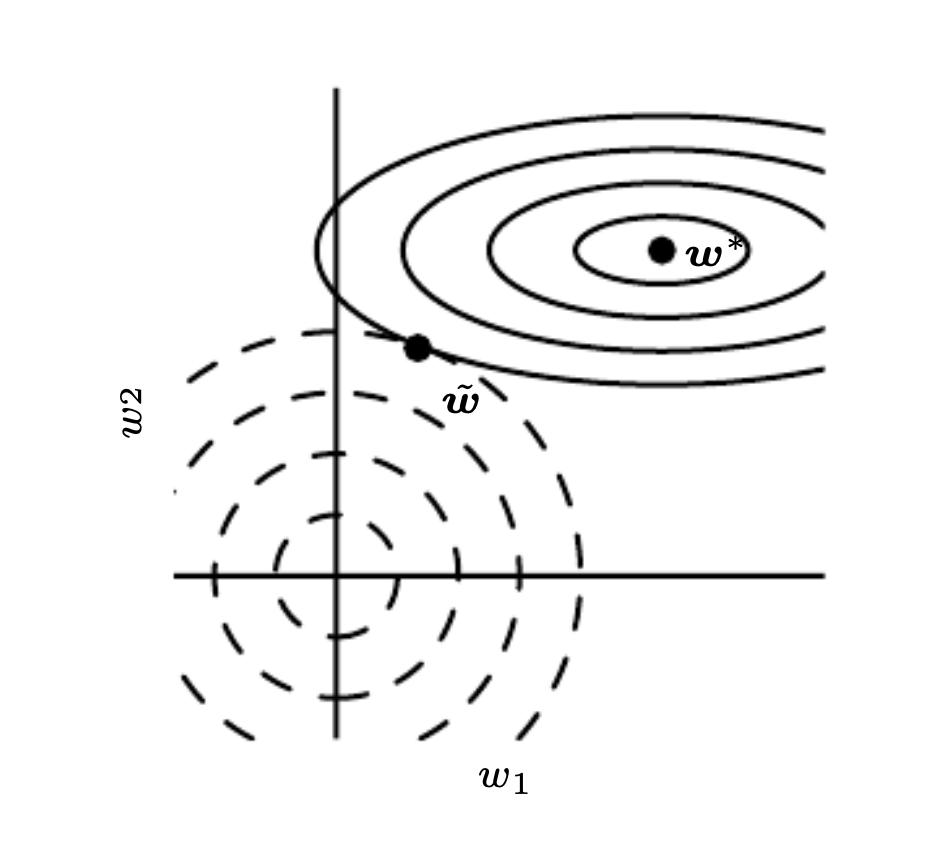
\includegraphics[width=0.3\textwidth]{plots/regularizedRegression.png}
\caption{Goodfellow et all, Deep Learning, p.~229}
\end{figure}
\end{frame}



\begin{vbframe}{Lasso Regression}
Another shrinkage method is the so-called \textbf{lasso regression},
which uses an \(L_1\) penalty\(^{(*)}\) on \(\theta\). We minimize:
\vspace{-0.1cm}
\[
\mathcal{R}_{lasso}(\theta) = \sum_{i=1}^n (\yi - \theta^T \xi)^2 + \lambda ||\theta||_1
\]
Note that optimization becomes harder now, because the problem is not
differentiable anymore.
$^{(*)}$ The $L_1$ norm is $||\theta||_1 = |\theta_1| + |\theta_2| + ... + |\theta_p|$
\vspace{-0.1cm}
\begin{figure}
\center
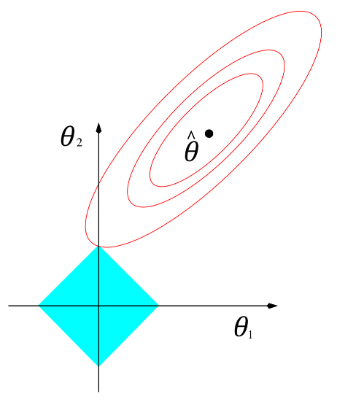
\includegraphics[width=0.3\textwidth]{plots/lasso.png}\\
\end{figure}
\end{vbframe}


\begin{frame}{Ridge vs.~Lasso Regression}
\textbf{Sparsity of the solution}:
\begin{itemize}
\item Lasso regression ensures a \textbf{sparse} solution (it selects features)
\item Ridge regression includes all features
\end{itemize}

\textbf{High-dimensional feature spaces} (\(p \gg n\)):

\begin{itemize}
\item Lasso selects at most \(n\) features (even if more features are associated with the target)
\item Ridge regression performs well in high-dimensional feature spaces
\end{itemize}

\textbf{Correlated features}:

\begin{itemize}
\item If features are highly correlated, lasso selects only one of these and ignores the others
\end{itemize}

Observation: Adding a regularization term to the loss has an high influence on the final model.
\end{frame}


\begin{vbframe}{Example: Polynomial Ridge Regression}
Again, let us consider a \(d\)th-order polynomial
\[ f(x) = \theta_0 + \theta_1 x + \cdots + \theta_d x^d = \sum_{j = 0}^{d} \theta_j x^j\text{} \]

True relationship is \(f(x) = 5 + 2x +10x^2 - 2x^3 + \epsilon\)
We saw. that a linear model  with \(d = 10\) tends to overfit:

\begin{figure}
\center
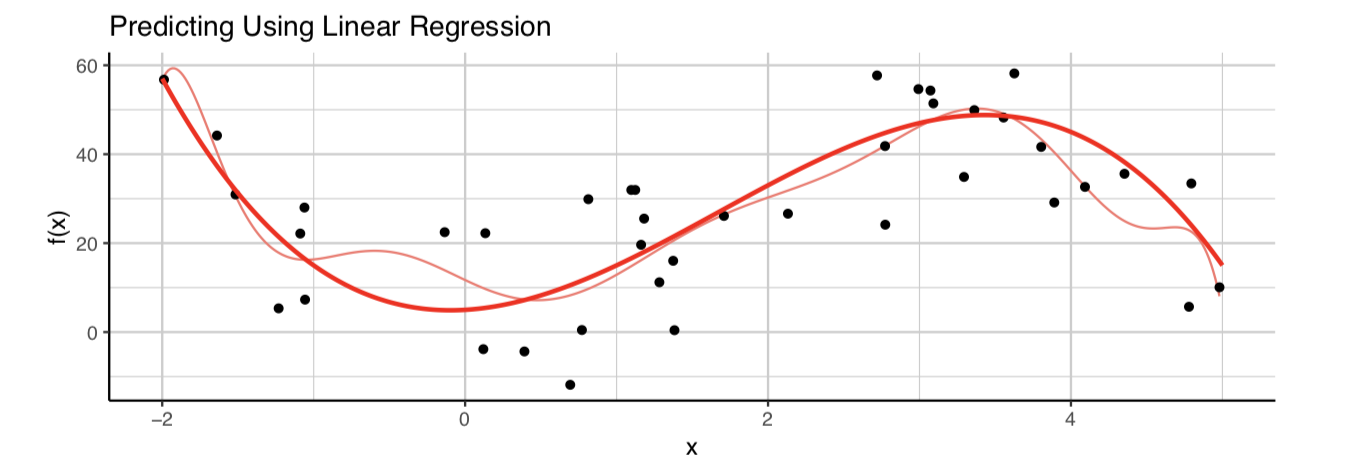
\includegraphics[width=0.9\textwidth]{plots/ex_linearRegression.png}\\
\end{figure}

\framebreak

Using ridge regression with suitable \textbf{regularization parameter}  $\lambda$ leads to better approximations of the data generating process.

\vfill

\begin{figure}
\center
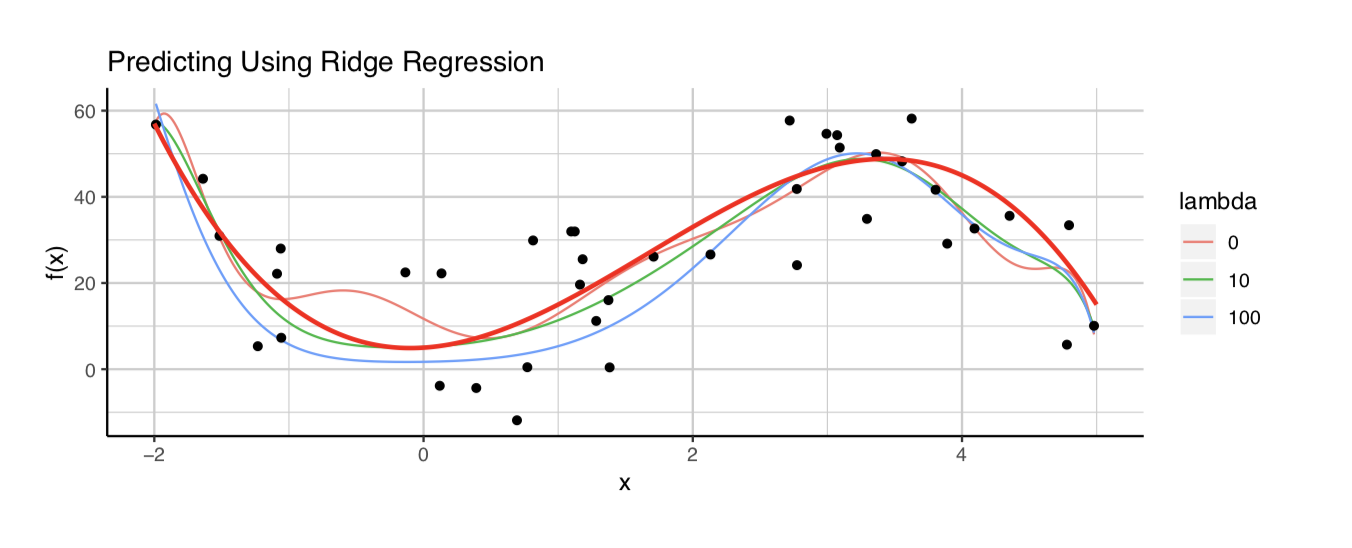
\includegraphics[width=0.9\textwidth]{plots/ex_ridgeRegression.png}\\
\end{figure}
\end{vbframe}


\begin{frame}{Example: Regularized Logistic Regression}
We can also add a regularizer to the risk of logistic regression

\begin{align*}
\riskrt &= \risket + \lambda \cdot J(\theta) \\
&= 
\prod_{i=1}^n  \tau(\theta^T x)^{y^{(i)}} [1 -  \tau(\theta^T x)]^{1 - y^{(i)}}
+ \lambda \cdot J(\theta)
\end{align*}
\end{frame}


\begin{frame}{Example: Regularized Logistic Regression}
We fit a logistic regression model using polynomial features for \(x_1\)
and \(x_2\) with maximum degree of \(7\). We add an L2 penalty. We
see
\begin{itemize}
\item \(\lambda = 0\): the unregularized model seems to overfit
\item \(\lambda = 0.0001\): regularization helps to learn the underlying mechanism
\item \(\lambda = 1\) displays the real data generating process very well
\end{itemize}
\begin{figure}
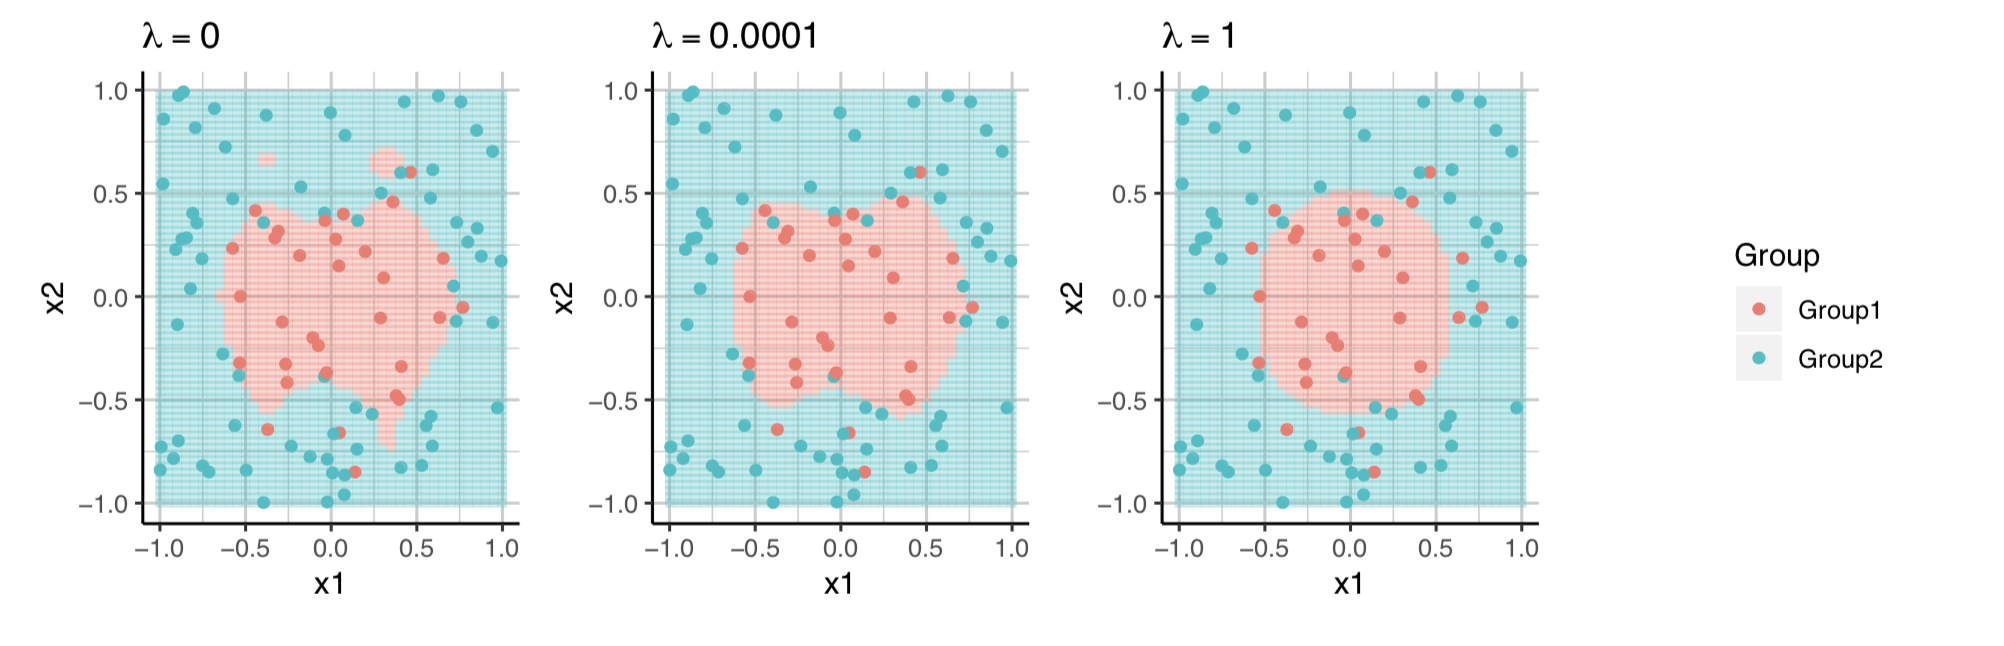
\includegraphics[width=0.9\textwidth]{plots/regularizedLogReg.png}
\end{figure}

\end{frame}


\begin{frame}{Regularization}
We now generalize the concept of regularization:
\begin{itemize}
\item Instead of linear nodel, any model \(f\) could be considered
\item Instead of the MSE, any loss function \(L\) can be considered
\item Instead of the \(L_1\) or \(L_2\) penalty and \textbf{complexity penalty} or
  \textbf{regularizer} \(J(\theta)\) can be considers 
\end{itemize}

\[
\riskrt = \risket + \lambda \cdot J(\theta)
\]

\end{frame}


\begin{frame}{Regularization}

\begin{center}
\begin{figure}
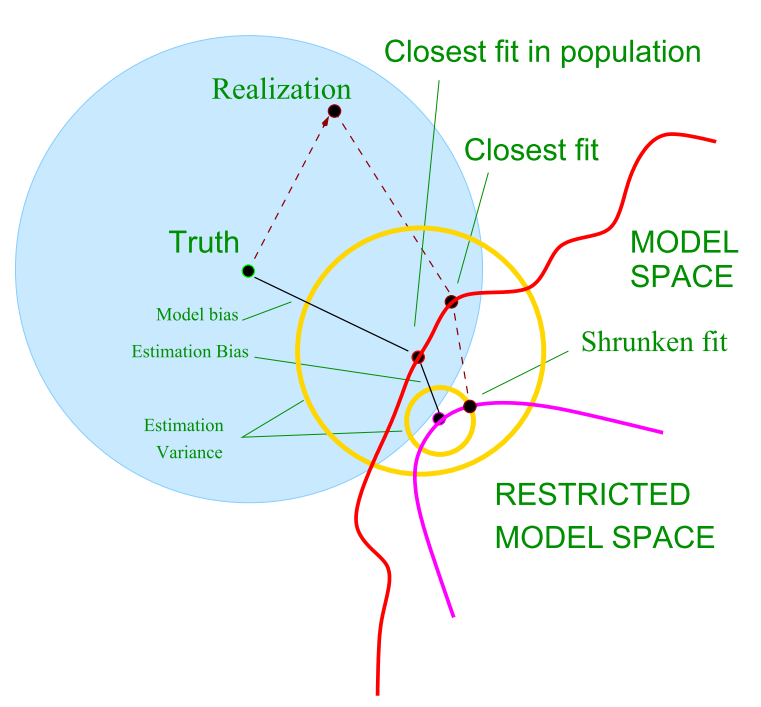
\includegraphics[width=0.6\textwidth]{plots/biasvariance_scheme.png}
\caption{\footnotesize{Hastie, The Elements of Statistical Learning, 2009}}
\end{figure}
\end{center}

\end{frame}

\begin{frame}{Regularized Risk Minimization}
We now have extreme flexibility to make appropriate choices in
\(\riskr\): \[
\riskrt = \sumin \Lxyit + \lambda \cdot J(\theta)
\]

\begin{itemize}
\item the \textbf{model structure} for \(f\), affects how features influence \(y\)
\item the \textbf{loss function} that measures how error should be treated
\item \textbf{regularization} \(J(\theta)\) that encodes our inductive bias and preference for certain simpler models
\end{itemize}

\end{frame}


\begin{frame}{Further Comments}
\begin{itemize}
\item Note that very often we do not include $\theta_0$ in the penalty term $J(\theta)$ (but this can be implementation-dependent)
\item These methods are not equivariant under scaling of the inputs, so one usually standardizes the features
\item The regularization parameter \(\lambda\) is a hyperparameter that needs
to be chosen carefully. One way  to tune it  is cross-validation
\end{itemize}
\end{frame}



\begin{vbframe}{Regularized Risk Minimization and Bayes}
We have already created a link between maximum likelihood estimation and empirical risk minimization. How about regularized risk minimization?

\lz

Assume we have a parametrized distribution $p(x | \theta)$ for our data and a prior $p(\theta)$ over our parameter space, all in the Bayesian framework.
From Bayes theorem follows:
$$
p(\theta | x) = \frac{p(x | \theta) p(\theta) }{p(x)} \propto p(x | \theta) p(\theta)
$$

\framebreak

The \emph{maximum a-posterio} (MAP)  estimator of $\theta$ is  defined as the minimizer of
\vspace{-0.2cm}
$$
- \sumin \log p(\xi | \theta) - \log p(\theta).
$$

Again, we identify the loss $\Lxyt$ with $-\log(p(x | \theta))$. If $p(\theta)$ is constant, so we have a uniform, non-informative prior, we again arrive at empirical risk minimization.

\lz

If not, we can identify $-log(p(\theta))$, our prior, with our regularizer $J(\theta)$.
If we introduce a further control constant $\lambda$ in front of the prior,
we arrive at regularized risk minimization.

\lz

Example: Rigde regression with linear model $\fxt$
\begin{itemize}
\item L2 loss = normal distribution of error terms
\item L2 regularizer = Gaussian prior on $\theta$
\end{itemize}

\end{vbframe}


\begin{frame}{Summary}
\begin{itemize}
\item A performance measure is applied to evaluate a trained model
\item We saw different measures for different tasks, sometimes they match the loss
\item Not the training error, the generalization performance counts
\item One can estimate it by evaluating the model on a hold-out data set (i.e. a test data set) or via cross validation
\item  Overfitting: model may over-adapt to the training data
\item Overfitting can be avoided by using more training data, early stopping, restricting the hypothesis class or other forms of regularization
\item In reguralized risk minimization a complexity penalty is added to the loss function, e.g. in ridge and lasso regression
\item From a Bayesian perspective, the reguralizer can be identified as a prior

\end{itemize}
\end{frame}


\endlecture
\end{document}